\documentclass[twoside]{book}
\usepackage{xspace}
\usepackage{url}
\usepackage{graphicx}
\usepackage{float}
\usepackage{lastpage}
\usepackage{makeidx}
\usepackage[myheadings]{fullpage}
\usepackage{verbatim}
\usepackage{fancyvrb}
\usepackage{amsmath, amsthm, amssymb}
\usepackage{fancyhdr}
\usepackage{xcolor}
\usepackage{pdfpages}
\usepackage[xetex,bookmarks=true,pagebackref=true,linktocpage=true]{hyperref}
\usepackage{adjustbox}

\usepackage[paperwidth=5.5in,paperheight=8.5in]{geometry}

\renewcommand{\thefootnote}{*}

%% figure placement
\renewcommand{\topfraction}{0.85}
\renewcommand{\bottomfraction}{0.85}
\renewcommand{\textfraction}{0.15}
\renewcommand{\floatpagefraction}{0.8}
\renewcommand{\textfraction}{0.1}
\setlength{\floatsep}{5pt plus 2pt minus 2pt}
\setlength{\textfloatsep}{5pt plus 2pt minus 2pt}
\setlength{\intextsep}{5pt plus 2pt minus 2pt}

%% \setlength{\textwidth}{340pt}
%% \setlength{\textheight}{502pt}

% fonts
\usepackage{fontspec}
\usepackage{xunicode}
\usepackage{xltxtra}
\defaultfontfeatures{Mapping=tex-text}
\setmainfont[]{Minion Pro}
\setsansfont[]{Myriad Pro}
%% \setmonofont[Scale=0.85]{Courier}
\usepackage{sectsty}
\allsectionsfont{\sffamily}


\title{Ergo}
\author{Ian Millington}
\date{November 7, 1999}                                           % Activate to display a given date or no date

\begin{document}
\maketitle


With thanks to Richard Northedge, Paul Hughes, Geoff
Millington, Rose Millington, Matt Rogers, Sian Lewis,
Melanie Millington, Andy Wood, Greg Scott-Cook, Graeme
McClelland, Contributors to rec.games.design.

This book is released under the Creative Commons Universal license.

\tableofcontents

\chapter{Preface}

This book is written in the style of a commercial role-playing product. This
is a stylistic choice. It isn't intended to be a commercial role-playing
game, but an experimental work in progress. 

%% TODO: mark these as such:
%% I have denoted sections or chapters which are very esoteric with one, or
%% in rare cases two, asterisks. 

Treat all pronouncements on the rights and wrongs of role-playing as much
more tentative than they appear. Most decrees in this book are actually
inferences made from thinking about collaborative role-playing and what it
would entail.

The style of the text is probably too ponderous, formal and
academic. This is not a bad this as the experience of writing a
sizeable piece of work like this was a warm up for writing my
doctorate thesis in science. The more academic and unreadable this is,
the better the warm up!

The critical section of the work is part one which describes my
collaborative role-playing in general. The rule mechanics in section
are intended to support collaborative style play but are not what the
game is about.

Comments, criticisms and especially suggestions are welcome on any
aspect of Ergo. Nothing here is written in stone and nothing should be
considered unchangeable. Email your comments and suggestions to
{\tt ian@agon.com}.

A convention has been maintained in these rules to use the female
pronoun and female names to refer to players, and the male pronoun and
male names to refer to characters in the game narrative. This is
intended for clarity, not to indicate the intended audience or
limitations on the game.
% \section{A note for this plain text version. }

% The `depth' of a heading is indicated by the number of blank lines
% preceeding it. Three blank lines represents a chapter heading, two for
% a section heading, and one denotes a subsection heading.

\chapter{The World Needs a New RPG Like...}

Role-playing games are ten a penny, role-players are a dwindling
breed. Most role-players are intelligent and fairly studious, and
almost all are partial to creating their own rules if not whole
systems. There must surely be more role-playing games than
role-players.

\section{A Jaded History of Role-Playing Games\protect\footnote{This section is {\it somewhat} esoteric.}} 

People play role-playing games to have fun. The first aim of any
role-playing can only be to facilitate fun. The first role-playing
games sold well because of that reason - people had fun playing
them. Then new role-playing games came out because there were problems
with the first batch. Then players realized that playing role-playing
games was the fun bit, not just playing a particular role-playing
game. This gave rise to lots of mediocre, similar games (usually
growing more and more realistic, pedantic and complex). A new game was
not released because it was more fun than others, but because people
loved role-playing games, and writing a game gave you a share of the
market.

Then computer games came to a fore, the role-playing game market
collapsed, and the only new role-playing games that succeeded were
based on beautifully crafted settings. Role-playing was no longer
successful as an end in itself, players wanted to role-play in order
to have more and different control over the flow of a narrative
describing a rich, detailed and aesthetically pleasing setting. The
role-playing format has remained unchanged since the first games. Live
action role-playing aside, you could watch a group of gamers play for
hours and have no idea whether they were enjoying a quick session of
Chainmail, the latest epic Cthulhu campaign, or some hybrid game of
the gamesmaster's own devising.

\section{Ergo Sum (Therefore I Am...)}

Ergo is a different direction in the way role-playing games are
played. It changes the fundamental make up of a role-playing game by
making one simple change. In Ergo there is no gamesmaster, the players
get on just fine on their own. They collaborate and co-operate. There
is no adversarial gamesmaster whose evil plans need to be thwarted and
adventures need to be beaten.

Ergo does not have its own rule set. The concepts and mechanisms can
be used with any set of role-playing rules. Some rule systems will be
easier to use without a gamesmaster than others. Ergo was written with
a modified version of the FUDGE role-playing rules in mind. An
appendix may add optional FUDGE rules to aid collaborative
role-playing.

\section{The Basic Principles}

Collaborative role-playing is based on some simple principles:

\begin{enumerate}
\begin{item}
All players take responsibility for the game, both the
   game-mechanics and the flow of the story. There isn't one player
   with special powers whose word goes.
\end{item}

\begin{item} Characters are no longer the `avatars' of their players; i.e. a
   character is not some extension of the player into the
   gamesmaster's world. Characters are actors in the story, the whole
   story is an expression of the players personalities.
\end{item}

\begin{item} Players are free to have more than one character, ebbing an flowing
   between them as the story dictates. Characters might have a
   `parent' player (called the character's guide) but can just as
   easily be shared or loaned to other players.
\end{item}

\begin{item} There is no such thing as player-characters and non-player
   characters, there are only characters. The evil pirate from one
   game might become a central character for a player in the
   next. Characters exist to be role-played, not as a player's only
   access to the game world.
\end{item}

\begin{item} Free from the need to win, role-playing becomes much more
   vibrant. Is a character more intelligent than its player? No
   problem, a player can role-play them in that way because the player
   also controls the setting. Would a character run away in the heat
   of battle? Now you won't be stuck out of the game if you let your
   character do exactly that. Players can get a much better sense of
   their characters as complete beings.
\end{item}

\begin{item} Players can organize role-playing in much more flexible ways. Many
   overlaying plots can be set up with overlapping characters. Two
   players go hiking for a weekend and a whole new backstory is
   born. The other three players send round a few emails, and a rumor
   from an unheard of race drifts into the storyline...
\end{item}

\begin{item} There are no barriers on the speed, format or medium in which the
   game is played. It is as suited to one long email per week as it is
   to an afternoon of round-the-table play. A painting is a
   contribution in the same way as a dialog between two characters or
   a description of a haunted mansion. The game works even when
   different mechanisms of communication and expression are used at
   the same time.
\end{item}

\begin{item} Ergo is a game, not a framework for collaborative writing, or a
   tool for making really detailed settings. There is at least as much
   role-playing, problem solving, exploration, and adventure as in any
   other game. More so when you consider that now everyone gets to do
   everything.
\end{item}

\begin{item} The narrative of the game is the central focus. All players
   collaborate to make the most exciting, beautiful, and tangible
   narrative possible.
\end{item}

\begin{item} Collaboration requires players to have good inter-personal
    skills. Everyone has the same goal: to have fun. Success comes
    from adding a second goal: to help everyone else have fun. There
    may be disagreements, inconsistencies, and perhaps even some bad
    feeling. Out of this a group of good imaginative players will
    forge a role-playing game deeper and more memorable than is
    possible in conventional play.
\end{item}
\end{enumerate}

\section{Setting and Mechanics}

Ergo is designed to be genre-neutral. There is no material here that
explores a game setting, or gives rules to help re-enact the fantasies
of some author. The game can be played in any genre and in any
setting.

That is not to say that all genres and settings will be equally well
catered for by this game. These rules are designed with the most
popular role-playing genres in mind: fantasy, science-fiction,
cyberpunk, gothic and modern horror, superheroes and historical
fiction. You may find them completely unsuitable for playing cartoon
characters or for your epic bacterium role-playing game set in a dog's
small intestine. Choose games mechanics that are reasonably
simple. You will be creating lots of characters on the fly, so the
main requirement is that you should be able to create sketchy
characters very quickly. A gamesmaster has the luxury of being able to
plan non-player characters in advance. This slows down a collaborative
game.

The notion of collaborative role-playing makes some types of scenario
difficult to play convincingly. Similarly there are types of scenarios
that you will come to love playing collaboratively that are impossible
with a gamesmaster. It will almost certainly not work if you try to
collaboratively play through an off-the-shelf adventure designed for a
gamesmaster to run.

Collaborative role-playing is better suited to games that are a little
`higher' on the realistic to epic scale. The central characters
benefit from being fairly powerful relative to the average person in
the game world. Games involving exploration of dungeons don't work
well, but if the main characters were competing dungeon designers in
the custom-lairs-for-vicious-tyrants industry, then the game could
develop interestingly. In general if the only point of the story is
for characters to find out relatively simple information (like the
layout and contents of a cave system), then boredom may
result. Exploration games can still work, but the thing being explored
must be interesting enough that players can have fun creating it while
their characters are exploring it.

Designing games to play collaboratively is a little different from
designing conventional scenarios. You have far more flexibility, but
Ergo doesn't stop you creating a terrible adventure.

The general style of role-playing advocated here should be completely
game-neutral. You can take the good ideas and go right back to your
favorite system to apply them. The mechanics for the game are
designed to help players play collaboratively and to remove all trace
of the player/gamesmaster divide found in many other systems. But if
you always play in one system, and you know it like the back of your
hand; use it.

Hopefully if you decide not to play collaboratively, you will still
find that the collaborative ethos filters down to your normal
play. Why not have the players to look up the damage they do to an NPC
and describe what it looks like? Why have folks tell the gamesmaster
the player's intent when they can use the mechanics themselves to find
the result? Let them tell everyone the character's actions!

In short Ergo is designed to be as flexible as possible. It is a game
system that promotes collaborative role-playing. Use it as you see
fit.

\chapter{Anatomy of a Game}

Your experience of role-playing is probably based on experiences of
playing with a gamesmaster. To play collaboratively takes a change in
mind-set. No longer is there one player with control over the game,
everyone must share that control in a co-operative way. With no
`higher authority' to appeal to, it is easy to get option paralysis or
to see the game as amorphous and pointless. It is worth bearing in
mind that people new to role-playing games often feel this way about
games with a gamesmaster. We are used to our board games having strict
inflexible rules, as barriers are removed we lose a grasp on what
moves we can make and what we need to do to win.

To make sure the game does not drift off into the playground game of
`let's pretend', there is some skeleton structure that can be imposed
on play. This helps everyone to see what they are doing, what the
goals are, and what kind of possibilities are open.

The raw materials of the narrative are divided into setting and
characters. There are some overlaps here; a character may be such a
background force that he merges into the setting, or some object seems
to have a life and character of its own. It is convenient to think in
terms of characters; things that can be role-played, and setting;
which provides the scenery, background and history for the
narrative. This is a static division, it doesn't say how the narrative
progresses.

The way the narrative progresses is broken down into playable
pieces. Small elements of the story are put together to make larger
and larger units. The most important result is that characters, the
focus of any role-playing game, are placed definitely in these story
elements in a way that lets players get hold of them and role-play.

The smallest unit in the narrative is a tactical situation. This is
roughly equivalent to a scene in a play or novel, or an encounter in
some other role-playing games. Tactical situations involve some set of
the characters in the story. Some may leave or join the scene as it
progresses, but it has some point for the characters involved.

Tactical situations are sometimes linked together to form plots. A
plot is part of the narrative that deals with a small number (often
one) character. Each character's plot may be completely different,
intricately connected, or permanently fused with the others. Plots can
be played as a set of tactical situations involving common characters.

Overlaid onto plots are strategic situations. A strategic situation
roughly corresponds to a long chapter in a novel, or an act in a stage
play. Some stories may only consist of one strategic situation, others
may be formed from a long set, all inter-connected. Most fiction is
organized so that strategic situations are played out in chronological
sequence. This may involve a plot coming and going over time. You
could decide to play through each character's plots in turn, letting
the strategic situations ebb and flow. It is possible, but may prove
unacceptably confusing and prone to inconsistency.

\section{Setting}

The setting of the game is all the extra information about the game
world needed to role-play its characters properly. A game's setting
can consist of the history, geography, myths and legends, technology,
languages, races, species and magic of a world, among many other
things. Most game settings will have some kind of map, probably a
background story, and some indication of the kinds of technologies
available.

The most general kind of setting is a game genre. There are
conventions in genres that help us to take for granted lots of the
setting material. Playing a game in the cyberpunk genre, for example,
probably means that characters have access to powered vehicles,
firearms and industrial cities. An important part of a genre, and the
whole setting of a game, is its mood. What kinds of emotions are
aroused when thinking about the world? What kinds of feelings motivate
its characters?

The setting for a conventional role-playing game is the sole
responsibility of the gamesmaster. She prepares material, designs
histories and draws maps. This may be made easier by using published
scenarios, but hers is the final word. Collaborative role-playing
demands that everyone shares the task of making a successful setting.

To avoid everyone designing the same thing in a different way, it is
more successful to allow players to take on sections of the world,
either geographical or social, and concentrate on their creation. The
more your group of players likes to develop complex settings, the more
it is important to communicate what each person has done or is
planning to do. This doesn't mean everyone has to know everything. In
fact that would make a very dull game. It should be clear the general
sphere each person is working in. This can be as simple as `I have a
city about here on the map.' Approach this process in a hands-off
way. If a player wants to create something, then let her. If isn't
quite what you imagined, then tough - collaboration takes you beyond
your own imagination.

To start playing a completely new game, a fair amount of setting
design needs to be carried out before play begins. Do not overestimate
the importance of this; part of the game will be to add detail and
complexity to the setting during play. It is one of the strengths of
collaborative role-playing that the setting can evolve a great deal
during play. Often decisions have to be made in the course of a game
that have large scale effects on the whole setting. The mood of the
game is one particular area that should be allowed to evolve. With
different players creating different aspects of the world, there will
be powerful changes and contrasts of mood; very much like the real
world, but unlike most role-playing games.

Lots of work can be done on the game setting outside of a play
session. Players aren't restricted to developing their character
background (although that too is important), they can create new
cities, devise archaic legends, hideous cults, starship manufacturers,
or underground revolutionaries. If you are stuck, then consider adding
depth to characters that are important to you. Why not think about
what life is like for the peasants working the fields around your
knight's castle, or how the surrounding countryside is laid out to
help the annual hunt? Why not host the annual hunt, as background?
Then when other characters turn up at the castle in three weeks time
for a parley you will know that wild-bore not beef is on the menu. You
know that's what was caught this year in the surrounding woods and
that is what is on the table. From this kind of little detail a rich
and elegant setting is formed.

Some players prefer not to spend all their spare time working on game
settings, however. Collaborative role-playing is at its strongest when
player's differences are respected. Resist the temptation to fill in
someone else's details for them. If one player's section of the map is
sketchy, why not reflect this in the game? The galaxy beyond the
nebula where strange rumors abound and maps never seem to
agree. Another player has penchant for writing reams of detailed
background, why not use this in the story? The city-wide vampire
brotherhood that was so bent on maintaining orthodoxy that it wrote
down all its history, rites and customs for acolytes to learn
thoroughly.

Allow the setting to have different facets and levels of detail. Each
player should try to develop settings in line with their personality
and approach to the game. The narrative will benefit from a lack of
uniformity.

\section{Character}

Characters are the focal point of any narrative. They drive the story,
interact, bring purpose to the setting and most of all make the
players care about the game.

Conventional role-playing games give each player one character to play
throughout the game. This has the advantage that the player gets to
know lots about the character and begins to understand what makes them
tick. It allows them to role-play the character in realistic and
interesting ways. The major disadvantage of this approach is that the
character is the only way the player can have any say in the game. The
characters actions not only serve to develop the character but are
also the players `moves' in the game, helping her towards a win. This
type of character, one that acts is a thinly veiled extension of the
player into the game world, is called an avatar, and it is a type of
character that Ergo tries to avoid.

In a collaborative game, players no longer need to have characters
that are their avatars in the game world. If a player wishes to act to
change the narrative then they can do so directly; they are partly
responsible for it, after all. Characters are used by players to tell
the story, to add richness and interest to the game.

With no gamesmaster, there is no difference between player-characters
and non player-characters. Different characters will have different
impacts on the story. Some characters will take the lead roles in the
narrative, while others will come and go like the extras in a
film. Normally each player will take sole responsibility for one or
two lead characters, they will create them, flesh out their background
and develop any connected bits of setting. This kind of player is
called the character's `guide'.

This is not to say that players can't share the lead characters
between them. It is a good idea to adopt the rule, however, that a
player should ask a character's guide before she starts playing him in
the game. People inevitably, and quite rightly, feel attached to their
lead characters, and having a definite guide for each helps avoid bad
feeling.

Most of the characters in the game will not have lead roles,
however. Less focal characters can have guides as well, but you will
find that there are lots of extras who should be played by anyone
convenient. Most of these extras never have any more detail than a
sketchy description and possibly a name; they are created on the spot
during play, and it makes no sense to assign them a guide.

You will probably find that a good balance is not hard to strike. Each
player will guide one or two major roles and several minor characters
(who they are more willing to share with others as the need
arises). There will then be a pool of communal characters, played by
anyone convenient as they wander in and out of the story. There
shouldn't be any one player who always plays the extras. At least one
player will normally have less to do in a situation than others, they
can fill in the minor characters.

Ergo characters can be developed in the same way as any other
role-playing game. Part of the fun in playing a character is
developing their background, motivations, customs and habits outside
the playing session. Players can work on their characters in the same
way. With some discussion, it is also possible for players to work on
aspects of other people's characters. One character may have been
close to another's parents and have knowledge of a deep family secret:
Does the other character know the secret? Should the player be told so
they can add flavor to their settings? Two characters might have been
squires together, a player can create background stories about both
character's time in service: Did they get into mischief? Does the
other player's character resent him because he never took the blame?
One character might have stolen another's spaceship: Are there
personal effects left inside? Is the other player out for revenge, or
happy with the insurance money?

Remember that you are free to develop the setting around a character
as well as their characterization. The possibilities for adding depth
and richness outside gaming sessions are unbounded.

\section{Tactical Situations}

Most of the playing time during a game session consists of tactical
situations. Characters are brought together in some part of the game
world to achieve a small goal as part of the larger narrative
sweep. Most role-playing games consist only of tactical situations,
connected into the larger storyline. The tactical situations in Ergo
likewise represent the basic unit of gaming.

Tactical situations can refer to anything from a short conversation
held between two characters in the street, to a hunting trip taken
over a week. It does not matter how long the situation lasts in game
terms. Tactical situations will typically have a small number of
characters in a small number of locations or settings. It should be
possible to play through one in a couple of hours maximum, sometimes
as little as a couple of minutes. This allows everyone to be focussed
on the purpose and conclusion of the situation and how it fits in to
the narrative.

Some examples of tactical situations might include: an interrogation
of a suspected criminal, chasing an arch-villain through Gotham city
(moving to a different tactical situation once they are caught),
trying to bluff a case of plutonium through Mars customs, the kings
annual jousting tournament, or an afternoon researching eldrich
horrors in the local library. Of course, each of these could be a
whole adventure in itself, but typically they will take an hour or so
of play, contain a small number of interacting characters, and enable
some definite conclusion to the situation.

Before play, everyone should have some idea of which characters are
involved in a tactical situation. Players will guide their own
characters, but also need to distribute responsibility for minor
characters and extras involved in the scene. The setting for a
tactical situation may be common enough that every player has a good
idea of what the scene looks and feels like. If the setting is
particularly associated with one player (she created this part of the
setting, for example), then that player might describe the setting,
the location and the atmosphere to the other players.

When one player sets the scene in this way, everyone needs to take
care not to think of them as a gamesmaster. Games where people take it
in turns to gamesmaster are rarely successful. When one player guides
a tactical situation, they bring their knowledge of the setting to
bear. Responsibility is still shared among all players, and the
setting should be allowed to evolve in response to player comments and
suggestions.

With the scene set for the tactical situation, players can then
role-play the characters they are controlling to play through it. The
actions of the characters should be allowed to mould and shape the
narrative. If there is a specific aim for the situation in terms of
the greater plot, be careful not to railroad the outcome to the
expected goal. If the exact result of a tactical situation is known
before playing, then play becomes trivial and boring. The interactions
of characters with each other and their settings can also inspire new
tactical situations and even new plots.

On the other hand a tactical situation should be a small section of
play, not a sprawling mess of events loosely tied to some
chronology. Because of the way players can split into smaller groups
to play Ergo, it is important to try to identify tactical situations
. Make sure everyone knows what the scene is, and in that way the play
can be concentrated on making the situation work. Every tactical
situation gives rise to many others that may or may not be played
out. Isolating the scenes from each other, especially while getting
use to other players' styles, makes everything cleaner.

One particular advantage of staying within tactical situations during
play, is that they can be easily documented in a few quick notes. Who
was present? Where did the situation happen? How did it end? A very
simple record of tactical play can help piece together the whole
narrative in player's minds.

Game situations which do not fit neatly into this model can still be
played; tactical situations shouldn't restrict possibilities. Play
does not only consist of tactical situations, just as conventional
games do not only consist of role-playing. Developing the setting and
story are important, as well as controlling the strategic actions of
the characters without having to play through their daily life.

\section{Plot}

Plots in Ergo are storylines that happen to characters. A character
may be involved in more than one plot at the same time. Plots
typically link all the characters in the narrative in an
interconnecting web of story.

Much of the plot might be created as part of the game setting,
character background or backstory. The rest is made up of events in
tactical situations. Typically plots don't need a whole lot of
collaborative development. They are not designed to define the story,
but to underpin character's activities. Plots should wind their way
through the lives of the central characters disappearing and
re-emerging later.

There are a lot of resources that can be used to come up with
interesting and powerful plots. In the early twentieth century
academic Georges Polti claimed he had discovered 36 fundamental plots
out of which all tragedy was built. This set of 36 plots makes an
excellent resource for deciding what kinds of plots to build your
narrative from and is discussed later in its own chapter. Not all
plots need to be terribly important to the characters involved. Some
things exist only as undercurrents, others linger and fester only to
erupt later, while still others are followed obsessively for while
before being completely forgotten.

For every character you control it is a good idea to know what plot
lines are affecting them, and which other characters are involved in
those plots as well. The more central the character, typically the
more plots they are involved with. Exceptions may occur. For example,
the local criminal mastermind may be a minor character, but central to
all nefarious plots in a city.

The complexity of the whole game is to some extent controlled by the
number of interrelated plots that are present in the narrative. If the
game becomes too complicated then let some plots die out completely,
if players wish to develop them further then they can do so as part of
their ongoing development of character and setting. If you choose to
drop plots completely, make sure you think through who will be
affected. It is easy to drop a plot without realizing that it is the
only link between two groups of characters in the world. Unless you
are willing to drop one of the sets you will have to split the whole
game into two.

Similarly if the game becomes to simple, or if a player finds one of
their characters too dull or isolated, then adding new plot lines can
be beneficial. When adding a plot line, take some time to think who
else would be good to link it to. Often some completely new minor
characters will need to be created to help the story along. It is
better to link two dull characters with a new plot than to create two
new plots. The intertwined branches of the story are what make Ergo
interesting to play; don't be afraid to make new connections between
characters.

Plots are an excellent way of developing different facets of a
character's personality. Characters should react differently to
different stimuli. If a character has several different plots they are
participating in, then it may be a good idea to let them show off
different aspects of the character's psyche. A character may be
involved in the upper echelons of organized crime, a plot in which
they are hard, cruel and callous. The same character learns his mother
has passed away, and the strong family sentiment he has comes to the
fore in grief and tears. Later his son wins a scholarship to the state
university, and he can't conceal his desire that the next generation
make something more of themselves than petty criminals. This kind of
overlaying personalities adds richness and believability to a
character, and also makes the character interesting to play. It is
easy to go too far down this road and make the character radically
different in each plot. This doesn't add depth, just effectively
increases the number of characters in the story. The character should
be, at the same time hard, callous, grief stricken and proud, the only
difference between plots being the degree to which each characteristic
is displayed.

\section{Strategic Situations}

It is not usual to play through one plot at a time. Plot lines tend to
come and go from the narrative over time. Games are normally played in
chronological order. Tactical situations played are in order of game
time. This means that it is impractical to play through one plot at a
time; this would mean lots of play out of sequence with a good
possibility that inconsistencies and impossible situations arise.

During play, tactical situations are grouped into strategic
situations, which are played in order. A strategic situation is like a
chapter of a novel or an act in a play; it advances lots of different
plots and sub-plots, but connects the individual scenes into some
logical whole.

Strategic situations are often built on one stretch of time, or all
the events in one larger activity. A strategic situation might
correspond to one day, or a week in the life of the characters, or
might be made up of all the events in a journey between two
cities. Geographical situations also make good groupings. The starship
Endeavour may find itself at a certain unexplored planet. The plots of
each character go on and may be explored in different details on this
particular mission; the captain's hatred of his engineering office,
the doctor's elicit affair with the weapon's officer's wife. The
strategic situation is to try to stop the planet being consumed by a
great fire. This introduces small mini-plots for characters; the
engineering officer must come up with a solution. These plots are
relevant only for this strategic situation, but are more interesting
if they can be merged into long term plots; the captain must put aside
his prejudices to rely on his engineering staff.

It is a good idea to try to identify the strategic situation that is
being played through. This helps all players get a sense of where the
game is going and what needs to be done. It also makes it much easier
to decide what tactical situations should be played. Role-playing is
inevitably about selecting what to play and what to leave out; nobody
plays through the actions of a character cooking beans on toast.  A
strong strategic situation will immediately suggest what obstacles
need to be overcome and what tactical situations should be explored in
depth.

A strategic situation can form one entire adventure. Short published
adventures for role-playing games do tend to consist only of one
strategic situation. Longer games can be made up of separate strategic
situations, possibly linked together with some common threads. Long
epic campaigns can consist of huge numbers of strategic situations
forming storylines that encompass the whole game world. For a truly
interesting game, the plots involving major characters should run
through all strategic situations; they belong to the characters and
should move with them.

Isolated strategic situations lend themselves well to games which
involve irregular intense periods of play. A group can meet all day
and play through one strategic situation, reaching its conclusion and
moving on to another strategic situation in the next session. They
also allow players to opt out of parts of the narrative. If a player
can only make a few sessions, then they can be part of one strategic
situation and not the rest. In some games pairs of players can decide
to meet more often to play through other strategic situations in the
same game world as the larger game. This kind of modularity opens up
lots of possibilities. It can also make gaming complicated, and it is
wise to make notes on the strategic situations being played through
and how they relate to the overall narrative.

There are two principle types of game that can be built up from
strategic situations. The first is an episode based game. In common
with most television series, episode based games deliver a different
storyline in each episode. Normally the same main characters (or some
subset of the main characters) deal with a different situation each
time. This game lends itself well to occasional play, and to play by
different combinations of players at different times. In the best
tradition of series such as Star Trek or Hercules, the strategic
situation may be based on some location. The main characters may be
government agents, and each episode is one mission they are sent on;
or characters might be witch-finders, and each episode sees the
hunting down of a new coven. Episode based play depends less on
character's plots to give life and vitality to the game. The
storylines introduced in the episode give most of the interest. Plots
should not be neglected, however. Watch any successful television
series and you will identify recurring problems and situations that
appear in many, but rarely all, episodes: these are the plots.

The second type of strategic game is campaign-style. The campaign
style game uses strategic situations to further one larger, often
hidden storyline. The characters may not be aware of what the overall
storyline is, but over time the strategic situations lead into each
other to provide a greater story. Many fantasy novels are of this
type; the Lord of the Rings sees many strategic situations merging
into the story of middle earth and its struggle against evil. Quests
like Lord of the Rings are a clear example of campaign-style
play. Characters set out on some long journey in which they find
themselves in many distinct situations, such as being captured,
negotiating a dangerous area, rescuing friends, making allies and
joining battles. In a quest the strategic situations combine to lead
the characters towards some goal that they may not even be aware
of. Each strategic situation is based around some reversal or prospect
of progress. A reversal is an event that moves the characters
backwards in their quest; it should be overcome to make progress. A
prospect of progress is some opportunity to move forward in the quest
that needs to be attained.

There is an unclear dividing line between plots and strategic
situations, and between episode-based and campaign-style games. A plot
involving a character may be the primary story in a strategic
situation, or some strategic situation may be punctuated by others in
the same way as a plot. Episodes may link together to form some global
story that is better seen as a campaign, or a campaign may have
separate stages so unrelated that they are episodes in all but
name. Inevitably you will also find game situations that do not easily
fit into either of these categories. The point of the distinctions in
this section is not to constrain you, but to clarify planning and
play. By all means experiment with new structures, but remember, the
most boring game will arise when most players are confused and don't
see what the point of playing is. Dissecting your narrative into
characters and setting and into tactical situations, plot and
strategic situations will help everyone see what they are doing and
why. They make it easier to keep records of your game and really help
everyone get a sense of the big picture.

* * *

The components that make up the narrative are only part of the whole
story. Ergo is a game; it is played. Play can also be divided up, into
gaming sessions and into non-session play. Gaming sessions are where
most of the play takes place on tactical situations. Other play can
add depth to settings, flesh out historical events, and enhance
characterization.

The idea of a gaming session in Ergo is a little looser than in most
role-playing games. Ergo is designed to be played by a range of
different communication methods; face-to-face, by email, in chat
rooms, by telephone, by letter or any other way you can image (anyone
fancy running a game by pigeon?) Having indirect play through email,
letter or pigeon means that there is no such thing as a gaming
session, all play takes place in the same way.

\section{Session Play}

For most people role-playing involves meeting (face-to-face or online)
and playing for a block of time. This kind of gaming is called session
play. It involves having a large amount of contact with the other
players. People get a whole lot more communicating done face-to-face
in an hour or so than in months of emailing back and fore every day.

Session play is suited to playing through tactical situations. The
interaction between players as they their play characters is
vital. Tactical situations involve all the players; those who don't
have lead characters to play can take on extras or may help describing
the setting,

There are some guidelines for planning a gaming session that can help
the narrative develop well. Lots of role-playing groups have
occasional long gaming sessions. Try to plan before hand a strategic
situation that can be played through in the session. The session will
then have a definite end and everyone leaves feeling they have
achieved something. If all the members of your group are rarely
available at the same time, then having and episode-based game can
mean that different strategic situations can have different lead
characters. That way a player who has to miss a session will not miss
any significant events in their character's life.

If you have regular short gaming sessions, then a strategic situation
can last over many sessions. The extra communication from session to
session can make it feasible to plan the tactical situations that you
want to play through in that session. Starting a weekly session with a
fresh tactical situation you have been thinking of all week is a good
way to get going. Likewise try to end with a complete tactical
situation to bring some kind of resolution to the game. Some player's
prefer to leave games on a cliff-hanger. This adds an element of
suspense but often means that important information about who was
doing what is missed. There is no reason why the cliff-hanger can't
lie between two tactical situations; the crusading characters have
battled through the outer castle court and are about to enter the
inner sanctum of the necromancer...

In general try to maximize the benefit of being together and playing,
either face to face or virtually. Make it as exciting and action based
as possible. This means tactical situations.

You may wish to nominate a chairperson for a gaming session. The
chairperson moderates what goes on during a session. This is not the
same as a gamesmaster. The chairperson doesn't get to decree what goes
on in the game (no more than any other player does), but is
responsible for making sure that everyone knows what is going on. This
can be especially important in sessions where a number of tactical
situations are being resolved at the same time. It is the
chairperson's responsibility to make sure everyone knows the plan,
what is upcoming, and what everyone wants to drink! It may be a good
idea to have the same person chairing a session as will be the guide
for the game setting. This way the chairperson can estimate how long
tactical situations will take to resolve, and make sure everyone can
get involved. You may find it completely unnecessary to have a
chairperson at all, especially if your role-playing group are
naturally well organized.

\section{Inter-Session Play}

Most players like to think about the game and develop their characters
between games. This kind of inter-session play is vital to
collaborative role-playing. In a conventional game all the players
expect the gamesmaster to have put some thought into the next session
before people turn up to play. The locations the characters may visit,
they extras they might meet, and the new storylines that will be
explored, all should be thought through at some level.

Likewise in a game of Ergo some thought needs to be put into the game
between sessions, but instead of being the responsibility of the
gamesmaster it can be shared by more players. Inter-session play sets
the scene for the tactical situations played through the next time
everyone meets.

Communication in inter-session play is vital. Email is a great tool
for keeping all players abreast of what you are working on. There is
always more that can be done between sessions to extend part of the
setting. Feel free to develop as much or little as you wish. Some
players tend to generate large quantities of documentation, others
think in broader more abstract terms.

Some things that can be explored between sessions include: characters
and characterization, background history, setting information, making
props, soundtracks or player handouts, plans for tactical situations,
new plots and the development of existing plots, ideas and plans for
new episodes or twists in the campaign, and sharing information from
different tactical situations played by different players.

\subsection{Characters and Characterization}

Character development takes place away from the game in the minds of
players as much as through role-playing. It is always valuable to
think about the motivations, personalities, backgrounds and
plot-involvements of your characters. Some players like to draw
character sketches, others write detailed histories, others write
their character's favorite song, or author poems on their behalf. The
best role-playing comes from having three-dimensional characters.

Inter-session play is an ideal opportunity to create new
characters. Each tactical and strategic situation probably will
require new characters, which should ideally be created beforehand
(but often must be created on the spot). For this reason it is a good
idea to use a game mechanic where simple characters can be created
quickly.

\subsection{Setting Information}

In addition to creating information about your characters, widen your
thoughts to their surroundings and lifestyle. In Ergo players are free
to develop incidental settings in detail. If your character comes from
a distant forgotten moon, then you are free to create the moon in as
much detail as you like. Many players do this kind of thing as part of
their characterization in conventional role-playing games. The
difference in Ergo is that if you play for long enough, you are quite
likely to find the game passing through the forgotten moon, and your
setting to become entwined in the lives of many other characters.

When creating new setting information it is especially important to
make sure everyone knows what you are doing, so conflicts don't
arise. One easy solution is to split up responsibility for different
parts of the game setting before you first start to play. The game
will always wander into unanticipated areas, but it takes no time at
all to assign parts of the new frontier to players who are interested
in expanding them.

\subsection{Props And Other Player Aids}

Many players love to have props such as newspaper articles, models of
sacred jewels, technical specifications for their spacecraft, and
threatening faxes from the games arch-villain. This kind of playing
assistance helps people role-play better. Since you will spend a good
proportion of the gaming time trying to think like your character, it
helps to have some of the things around you that they might
have. Props take a lot of work to produce, however, and should be
prepared before a session. All players can create props, but be
careful not to expect that other players will have as much time to
make an exact copy of the game's `Forbidden Tome of Age Old Priests'
as you.

Adding spice and richness to the game doesn't stop at making
props. Think about mood music. Can you bring along some background
music for one of the tactical situations that you are planning to play
through? Or why not agree with the players that each character should
have their own `theme' that can be played in the game when important
actions are carried out by that character. Creating the right mood can
extend beyond music; plan to play an important tactical situation in a
different place - on top a local hill, or in your garage. Have a
costume day when everyone dresses as their main
character. Inter-session play is the perfect opportunity for planning
to blur the lines between role-playing and acting.

\subsection{Session Planning$^\star$} % \protect\footnote{This section is {\it somewhat} esoteric.}}

Lots of valuable gaming time can be saved by planning at least the
first tactical situation for the next game session. Communicate with
the other players to work out what the tactical situation will be,
which characters will be involved, and where it will be set. Then when
the session begins, role-playing can begin straight away.

Plots also need to be planned, but can be developed by individual
players to a greater extent. Think of new plots to involve your
characters in, or ways to twist existing plots in and out of the
strategic situation. Before planning to incorporate a hundred new
plots into the next session, make sure everyone is laid back about
it. Weeding out old, tired plots for destruction or for a spruce up
will also add vitality to upcoming tactical situations.

Finally players need to talk about the next strategic situation and
how they see it being made up. In an episodic game, or a game where a
whole strategic situation is played in a session, this takes the place
of tactical planning. Players wont have as good a time if the
strategic situation isn't agreed until the session begins.

Planning the next session probably takes up the most time of
inter-session play. It can be the most fun too, building up lots of
anticipation for the big day when the tortuous situations stored up
for your characters will be let loose on them. The next chapter deals
with planning in more detail.

\subsection{Sharing Information$^\star$} %%\protect\footnote{This section is {\it somewhat} esoteric.}}

Very often groups of players will split off to play different tactical
situations in a game. This can occur as completely separate sessions,
or may just mean a half-hour in another room to everyone else. The
multilayered approach to collaborative role-playing is central to
Ergo, but it does introduce the possibility that the two tactical
situations running side-by-side will conflict. A separate section in
this book deals with mismatches and how to resolve them. Before you
can resolve a mismatch you need to know that one exists. This can only
be done if players communicate about what happened. In a session when
everyone is keen to get onto the next tactical situation this can be
inconvenient. Make sure that everyone gets the gist of your play
before the next session. That way large quantities of story wont be
built up on the mismatched parts of the game. There is nothing worse
than realizing you have played for weeks or months on the basis of
something that could not have happened.

\section{Indirect Play}

Indirect play takes place through letters, email or any other medium
that takes time to move between players. In indirect play there is
less opportunity for conversation, discussion or role-playing.

As remarked above, there is no such thing as a gaming session in
indirect play. The game moves on in the same way at all times. It is
still advantageous to think in terms of tactical and strategic
situations. Often whole tactical situations will be resolved by one
player in one email. Ergo allows players to take on whatever
characters they need to. One easy approach to indirect play is to have
a communal stock of characters. Players should briefly discuss the
next tactical situation to be played before allowing one player to
write a summary, or a short story based on what happens. The game can
develop in the same way, but players merge role-playing with setting
development into the same activity. Because of its shared
responsibility, collaborative role-playing is much better suited to
slow indirect play than conventional games.

With email play, a faster turnaround can be achieved and the game can
progress in almost the same way as in a face-to-face session. Make
sure everyone can get to their emails regularly, however. Two players
could launch into a quick exchange of email and leave other players to
find the results days later.

Indirect play provides excellent records of the game's progress. This
is a strength that can be used to add more subtlety to the game;
nobody can get lost with a complete record of the narrative.

\chapter{Playing a Game}

You are now familiar with all the components that go in to making up a
game of Ergo. Components are one thing, but the way they work together
in reality is another. Collaborative role-playing takes some getting
used to, and it can be difficult to image how the game will work. This
section steps you through all the bits of playing an Ergo game, from
the first ideas about genre and setting to the nitty-gritty of
resolving tactical situations.

The different activities involved in playing will vary from game to
game and from player to player. If you are intending to play a
pre-written scenario, then lots of the planning for the game will
already be done for you and you can skip straight to character
creation and then onto the game itself.

The different stages in playing the game are roughly: planning the
game, creating characters, setting up a strategic situation, deciding
on tactical situations, playing through a tactical situation,
expanding the game setting, and eventually playing a finale. You will
only have to plan the game once before you start playing, and you will
probably only want one game finale. All other bits will need to be
repeated as you play (unless your game is very short). This chapter
gives you an in depth insight into how to go about playing each stage
of the game.

\section{Planning the Game}

Typically a group of players will have worked out a lot about the game
they want to play before coming together to play. You may have decided
to play through a pre-written scenario, in which case you won't need
to plan the feel, setting and storyline for your game. Even if you are
starting from scratch you may have a feel for what genre or
combination of genres that the game will follow, and what is mood will
be. If you have not yet got this far, then this is where to start.

Once you have the feel of the game sorted, then you can sketch its
setting, a rough storyline and plan the opening strategic
situation. This information may already be provided for you by a
pre-written adventure.

\subsection{Game Feel}

The best way to get a handle on what you will be playing, as well as
making sure everyone knows what is going on, is to decide on a
definite genre (even if your game's genre is a little out of the
ordinary), how epic the game will be, and what kind of mood you want
to play for.

Decide what kind of game people want to play, and what kinds of
characters they want to control. You mix different traditional genres
together. How would superheroes handle life in the wild west? What
would happen if a medieval society used magic to develop space flight?
How would the pilgrims have coped if they found werewolves not native
Americans around Plymouth?

As far as role-playing are concerned, a genre is less a family of
similar works, and more of a shorthand for what can and can't happen
in a game. When players say that their game is `cyberpunk' then
assumptions about technologies, settings, character's and storylines
can be made. Of course, there's nothing to say that these assumptions
can't be challenged, but they provide a handy starting point.

It is wise at this stage to also decide how epic you game should
be. Highly epic games do not concern themselves with details and
realism. An epic game allows the hero to wade through the middle of a
firefight to pick up the wounded comrade, receiving only a rather
becoming scratch to the temple. Million-to-one chances happen nine
times out of ten. Epic games are sometimes referred to as `cinematic',
they work on broad sweeps of action rather than the small detail of
life.

In contrast a `low' game is concerned with being as real as
possible. A character that receives even a single gunshot wound will
probably die almost immediately. Million-to-one chances happen about
once in a million times, if ever. Low games are concerned with the
details of characters' activities, even if it is incidental to the
main story.

The third component in the game skeleton is mood. The mood of the game
is the type of emotion that playing should give rise to. Often the
mood goes hand in hand with the genre: horror games are often dark and
scary, space operas are often bright and optimistic and cartoon games
are usually humorous. Nothing is ever written in stone, and you can
easily mix and match to get your perfect blend. How about a cartoon
game which is brooding and serious, or comedy horror, or an black and
violent superhero / vigilante game?

Part of the feel in the game is generated by the way it is played. It
is a good idea to decide whether your game will have lots of strategic
situations or just one. If you decide that it will be a long game,
then you should also talk about whether to make it episode-based or
campaign-style.

When you can agree on genre, `epic-ness' and mood you are ready to
start filling in the broad brush strokes of your setting.

\subsection{Game Setting}

Your next task should be to decide on a setting for your game. If you
are not playing in a setting already devised (such as from a scenario,
book, or movie), then you will need to spend some time getting a
handle on what the environment will look like.

A lot of the setting will be suggested by the genre and mood in which
the game is set. If it is a gothic horror game, then it might be set
in Victorian England, with all its technologies and locations. A
science-fiction game will probably involve space-craft and computing
technologies.

Many players like to draw sketch maps of the world, or to write poems
or short stories set there. A quick list of major planets in a
science-fiction game, or some idea of the type of geography is
useful. If you are using real-world places, then decide if the place
should be accurate or improvised, and if accurate then in what era the
game is set.

You can add depth to the setting by talking about the game's history,
geography, myths and legends, technology, languages, races, species
and magic, among many other things. At this stage there is no need to
develop the setting in great depth. More detail will be added by
individual players and the real setting will build up over time as you
play the game. Making a sketch map, a few quick notes about history or
a short background story and some notes about the technologies allowed
should suffice.

\subsection{Rough Storyline}

Once you have a setting, it is a good idea to outline a rough story,
or premise for the game. This doesn't need to involve any characters,
although it will inevitably suggest some that need to be created. The
amount of detail that you can put into a storyline will depend on the
way you have chosen to play your game.

If you have decided on a episode-based game, then you should give an
indication of the story that links the episodes. The story will
inevitably be simple, since it won't change too much between
episodes. It can be as simple as `the main characters are paranormal
investigators working for the government; each episode is a different
case', or `after the nuclear war, fuel is scarce and the main
characters lead rival gangs moving between fuel dumps; each episode is
their conflict over a different dump'. From this basic story lots of
other decisions become easy: locations need to consist of fuel dumps
and their surroundings, characters need to be educated enough to be
recruited by government intelligence.

Quest-based games should also have a basic premise. In a
campaign-style game the story should describe the overall situation
that the campaign is trying to solve. The goals of the characters may
change as they learn more about what is happening in the world, but
the basic situation that required the quest will probably not change
very much. The storyline for a quest game might be something like `the
evil necromancer has plans to take over the world; he must be stopped
by the brotherhood of mages' or `the main characters accidentally fly
their spaceship through a black-hole and must try to find their way
home'.

Games that are only intended to have one strategic situation should
develop a storyline for it before players create their main
characters. The storyline for the whole game is the storyline for the
strategic situation. Before thinking about the strategic situation in
depth, however, it is still a good idea to come up with a simple
sentence that describes the point of the game. Details on how to plan
a strategic situation come later in this chapter.

From your rough storyline you should get a good idea of what the main
characters are going to be or what the goal of the game is. In an
episode-based game the characters are often the main unit that makes
all the episodes into one story. The characters might consists of a
group of friends, enemies, colleagues or competitors. In a
campaign-style game main characters are more likely to come and go
over the course of the game. The point of the game is often less
character based and more concerned with doing something (such as going
on a long quest) or managing something (like a secret cult or a
besieged castle). For campaign-based games, the goal of the game
should be decided. It might be to find some treasure, defeat some
enemy, maintain the status-quo or incite a revolution.

With a rough storyline, players should think about what main
characters need to be in the story, both protagonists and
antagonists. With a list of important characters, character creation
can begin.

\section{Character Creation}

Whereas you will only have to plan the game once before you start
playing, character creation will be an ongoing process throughout the
game.

Before you start playing it is important to create the main characters
involved in the story. These will be the characters that each player
will control most of the time. Because they are important characters,
they will created in some detail. You will also need to create the
antagonists of the story in some detail. Each strategic situation in
turn has its own cast of supporting roles that may spill over into the
rest of the game. These supporting characters tend to be created in
less detail, because their capabilities and background information are
less critical to the story. Finally new characters need to be
introduced in many tactical situations, these `extras' have little if
anything to do with the whole story, but function as bit parts shaping
the narrative. Extras need to be created in very broad brushstrokes,
rather than in great detail. In general main characters and some
supporting characters will belong to a specific player; the
character's guide. Extras can be played by anyone as required.

\subsection{Principal Characters}

The principal characters in a story are usually the protagonists;
those characters whose story it is. The protagonists are often the
heroes or heroines, but might equally be anti-heroes or heroines. Some
stories also require the antagonists, those individuals opposing the
actions of the protagonists, to take centre stage in the storyline. In
this case they may also be played as principal characters.

Character creation for principal characters should take place after
the planning stage for a new game. The principal characters tie the
whole story together and probably should be there to some extent
throughout the campaign. These characters may drop out, or die and
others take their place, but by and large they are a constant force in
the story. They are what gives the story personal focus.

Because principal characters are important in the game, and their
personalities give rise to much of the drama, it is a good idea to
have them played only by a single player. The character's guide can
then develop their background, motivations, personality and habits
without being distracted by other people interpretations. There is no
need for players' characters to all be friends or allies in the
game. A good story can be fueled by different factions of principal
characters, or even characters that are mutually opposed.

What is important for principal characters is that they are created in
some detail. This corresponds to the players' character creation
process in any other role-playing game. The principal characters
should be interesting enough to give rise to and sustain a number of
plot lines in the story, as well as being versatile enough to drive
the narrative and support good role-playing. They should be as near to
three-dimensional personalities as possible. Incorporate conflicting
motivations, irrational beliefs and unexpected emotions, after all:
those things are present in real people like you. On the other hand,
the aim of the game is to play collaboratively, so don't make your
character the embarrassing focus of the game by demanding attention
with wild displays of pointless emotion. Real people have lots of
conflict and subtlety, but it rarely peeks out from behind the normal
facade they foster.

During character creation you will inevitably find that the very
sketchy setting you designed while planning the game isn't detailed
enough to develop your character properly. This is intentional. Your
character will have experiences of their surroundings that couldn't
have been planned for even in if the setting were extremely
detailed. One of the great features of Ergo is that players develop
the setting, rather than the gamesmaster. Once you have outlined your
character you will find that you need to design some of the game
setting at the same time as the character. For example, you decide
that your character went to University, so you need to work out what
towns have a university, what they are called, what they are famous
for, and so on. Were their inter-varsity rivalries. Who had the best
magic faculty. Was your character involved when you kidnapped their
Football team's mascot? Or you might decide that your character comes
from a backwards, farming planet, but always hankered for adventure,
so you need to work out the planet's name, where it is located. Does
it trade at all? Would other characters know of it? What specific
skills did your character pick up as a farmer?

It is important, however, to make sure that you tell other players
which parts of the setting you are creating (but not everything you
have created). This avoids problems with different people designing
incompatible parts of the setting, or designing the same part of the
setting in completely different ways. The chapter on mismatches and
their resolution gives some hints on what to do if settings don't work
together.

It is also good to share an overview of your designs with other
players so they can use your ideas in their own character
creation. Two characters might have gone to the two rival
universities, for example. The more you use other players ideas to
extend your own the more the story will be woven together and the more
good opportunities will arise for interesting role-playing. The
section on expanding the setting, in this chapter, gives more advice
on how to add depth to the game's environment.

\subsection{Supporting Characters}

Creating principal characters and their settings in depth takes quite
a long time. Too long to spend on every character in the
story. Supporting characters have a smaller role in the story, and
players can afford to take less time creating them and their
background.

Supporting characters are often crucial to the story for only one
strategic situation, even though they may occasionally crop up
later. When planning a new strategic situation, supporting characters
must be considered and built.

Despite the fact that supporting characters are created in less detail
than principal characters, they still require some thought and
planning. In some cases new setting information will be needed,
although this should be kept to the minimum possible. Supporting
characters often belong to an individual player who creates and plays
them. Unlike principal characters, however, other players can take
control of the character in the game when needed. It is sometime
necessary to swap over play of supporting characters to suit a
particular tactical situation. If one player's principal character is
having a discussion with one of their supporting characters, it makes
little sense to have one player take both roles in the conversation
while other players have nothing to do.

Character creation for supporting characters should focus less on the
characters background and history and more on their capabilities and
personality. For the majority of supporting characters, the storyline
is too removed from them to delve deeply into their history and
setting. The important facets to concentrate on are the
characteristics that make them unique, and uniquely able to contribute
to the story.

One exception to this guideline is for supporting characters in an
episode based game. For the duration of one episode some supporting
characters may be at least as important as the principal characters,
if not more so. The backgrounds and motivations for these characters
often define the story in the episode, and need to be developed in
depth. Episodes can be so independent of each other that they are best
approached as mini-games in themselves, with the retention of a few
characters from a previous game. If the episodes in your game are
highly independent, then you will probably need to spend more time
between episodes planning the next strategic situation.

When creating the personality for a supporting character, try to make
it interesting and different from other characters. You should
probably not be aiming for a complete three-dimensional character,
however. The motivations for their actions should be obvious after a
few tactical situations are played through. Detailed conflicts and
histories make the character difficult to role-play effectively over a
small number of scenes, and may make it impossible to swap control of
the character between players. Aim for a two-dimensional character,
one who shows only one side of their personality in the game.

If a supporting character suddenly becomes very important to the
story, then their guide needs to spend some time fleshing them
out. Developing a three-dimensional personality, going back through
the character creation process and building a character background,
and detailing the settings that define the character's history all
should be done with care so that the new version of the character fits
seamlessly into the narrative. It is no good having a evil warlord who
tortures small puppies mellowing and joining the party, and instantly
adopting a pet dog. It is also important not to change the character's
characteristics too much. Some change is inevitable if the original
character was created in an ad hoc manner, but try always to retain
the essence of the characters abilities and gaps in ability.

\subsection{Extras}

Extras are simple characters that exist for a specific purpose in the
story. Extras often only pop-up in a single tactical situation; the
barman in a strange tavern, the trader at the market, the customs
official at lunar-immigration. Extras for the next tactical situation
are created regularly. They need to be quick to build, and very simple
to play. Spending time thinking about character background or rich
personalities is a waste when players are keen to role-play.

One approach to designing extras for the game is to develop stereotype
characters in advance. This can be done at the game planning stage or
when thinking about the strategic situation. The player responsible
for the setting in which the extras occur can produce one or more
generic characters with broad characteristics and abilities. This
might be as simple as one generic character for a new world that is
being visited, or a set of characters for each social status and
gender in a new kingdom. When an extra is needed in the game, the
generic character can be copied and one or two modifications can be
made to make the character fit their purpose in the story. The generic
planet-dweller can have the addition of some mental abilities to
become the immigration officer, the generic character gets some
physical skills to become one of the security guards in immigration,
and so on.

Building up a stock of generic characters can speed up the game to a
great extent. In some genres, however, the range of characteristics in
extras will be so great that generic characters will not save much
time at all. In this case extras need to be created from scratch as
they are needed.

Create extras from your knowledge of what characteristics they might
use in the upcoming tactical situation. Don't go through all the
abilities they may have, or how they got those abilities, just focus
on the why the extra exists in the story. If the extra is a barman,
then they should have bartending skills, but disregard the fact that
they ride horses in their spare time. If this kind of detail becomes
important, then you can spend more time making them into a good
supporting character later.

Extras should be one-dimensional, the briefest sketch of realism. Most
extras will have very little or no personality in the game, it is not
wise to spend lots of time giving them motivations and beliefs. If an
extra is to have some obvious personality trait, then make it a
caricature; some speech impediment, turn of phrase or accent. One
single defining point often sticks in the mind of players and can help
to define a tactical situation. Resist the temptation to give
everybody this kind of treatment. The story will rapidly descend into
farce if every character has a slightly different nervous twitch and
speech problem. This is not a problem, of course, if your story is
supposed to be a farce!

Keep a hold of your notes for the extras you create. The easiest way
to build generic characters is to keep previously created extras and
then modify them slightly. The barman at the next tavern is probably
similar to the last one, but a little better at conversation, say.

\subsection{Plotting for Characters\protect\footnote{$^\star$ This section is {\it very esoteric.}}$^\star$} %%} 

Regardless of the type of character that you are creating, you may
wish to consider what plots they are embroiled in. This is very easy
to do for extras, since they will probably be involved in only one
tactical situation, and so are connected to the story being played out
there.

Supporting characters can hold one or two major plot lines, which
should coincide with some of the plots of principal characters and
other supporting characters. Principal characters can support many
more plots, which can be independent of other characters as well as
woven together. Some of these plots may never be investigated in the
game, but help a player to understand the motivations of her
character.

Note down each plot associated with the character and which other
characters are also involved. If the plot is central to a strategic
situation then more details need to be given, and the plot should be
discussed between players. Otherwise a couple of sentences will give
enough detail to start playing and more information will come to light
over time.

\section{Planning a Strategic Situation}

Strategic situations are a convenient way to group parts of the
narrative into sections of game with their own storyline: opening,
development and ending. A strategic situation will have a consistent
setting and array of supporting characters. Before playing a strategic
situation, it is a good idea to get an idea of the story behind the
situation and how it might pan out through play. Strategic situations
are made up of tactical situations which go together as part of the
overall story.

Strategic situations can be thought of as mini-games in
themselves. Many games consists only of one strategic situation, it is
like a small adventure or scenario in a conventional role-playing
game. There is a definite goal, and the characters move towards that
goal overcoming difficulties on the way. The strategic situation may
be part of a larger story but should function as a mini-story in
itself. This is especially true in episode-based games where strategic
situations are even more important in story development. Collaborative
games work better highly modularized in this way. Strategic situations
give a focus to play and avoid the players facing option paralysis.

Another advantage of story modularity is that strategic situations can
be designed by a group of players, or even a single player. This works
better in episode-based games where there is little need for strategic
situations to integrate tightly into an overall story. The players
will act as the strategic situation's guides, and should probably be
responsible for designing the setting and supporting characters
too. This is as near to a gamesmaster as is allowable in Ergo.

Planning a strategic situation consists of developing a storyline,
adding the setting, creating supporting characters and deciding on a
few keyframes.

\subsection{Developing a Storyline}

The storyline for a strategic situation should be strong and
instant. It is the hook that defines this part of the game. There are
any number of different possible storylines for a strategic
situation. In general, however, the story should be defined around the
principal characters in some way.

Give the principal characters a definite goal in the situation. Some
criteria which shows when the strategic situation is over. This could
be a mystery to solve; find out who killed Baron Umberslade, for
example. It could be something to attain, such as bring the holy grail
out of the mysterious monastery. Or it could be a social problem to be
resolved, like preventing two planets declaring war on each other. The
goal is well defined. The characters don't need to know the goal, of
course, but the players designing the story do.

Once you have a definite goal for the characters to achieve you need
to have a hook to draw them in. The characters must have a good reason
for wanting to achieve the goal. Spending some time thinking of a good
reason that is out of the ordinary will add a lot to the game
play. Greed or curiosity are often used as a hook, but are not
particularly powerful, most people wouldn't risk their lives, for
example, because they were curious. Hooks can take the form of family
ties; one of the characters may be the son of Baron Umberslade. Duty,
honor or zealously are also powerful; there is no more noble cause
than to win the Holy Grail for one's king. Personal survival is
another great stalwart; the weaker warring planet is the characters
home, for example.

The best hooks are those that happen to the characters and embroil
them in the story with no option for them to weasel out. The
characters are more likely to investigate the demise of the Baron if
they are arrested for his murder than if he just happens to be a
friend of a friend. Storylines of escape, races against doom, mistaken
identity and natural disaster all have good hooks to draw in
characters.

Having a good hook also eases the process of designing the first few
tactical situations.

With a goal and a hook, the storyline needs some sketchy indication of
how characters might reach the goal. It is very easy to over write the
story here. Remember that playing through the strategic situation is
where the fun role-playing takes place. Strategic situations with only
one, tightly constrained path to the goal are boring to play and
easily forgotten. Ideally there should be at least three ways to reach
the goal. If you cannot think of three ways to reach the goal, then
the situation is probably too linear. Once you have a set of possible
routes to the goal, it is still important not to rely too much on your
three ideas. Remember that it will take much longer to play through
the situation than it does to plan, new avenues and approaches will
arise during play, and they shouldn't be ruled out by too strict
planning. In Ergo, remember, there is no gamesmaster, so the guide
cannot stop the players going in a new direction. Players are likely
to break through the walls of a linear plot and leave it in ruins.

The ideal storyline will have a strong concept, a well defined goal,
an inescapable hook and at least three loose possibilities for routes
to the goal.

\subsection{Adding the Setting}

The next step to developing the strategic situation is to add a
setting. Many storylines will immediately suggest a setting in the
game world. After playing through a number of strategic situations in
the game, the setting will be fairly well detailed and may suggest its
own strategic situations. If you don't have a definite setting in mind
you need to merge it into part of the setting for the game that has
already been developed, or create a new part of the setting to house
the story.

Using an existing part of the game setting has the advantage that it
reduces the amount of work that you need to do before the strategic
situation is ready to play. It also has the advantage of linking the
story in to previous parts of the narrative. Don't be limited to
setting stereotypes, either. It is even more effective to reuse bits
of settings in different contexts. If the characters has investigated
a ghost sighting at the renowned `haunted house', then make the next
ghost sighting at the railway station where they found the hobo with
strange powers, or in the school where one of the characters went as a
child.

The major disadvantage of reusing settings is that the storylines can
become stale and the game-play repetitive. It adds more spice and
excitement to explore new places and myths and meet new characters and
races.

If you decide to reuse an old setting, then try to add something to
it. Settings are like characters in more ways than is obvious at
first. Principal settings that underpin lots of the narrative should
be developed like principal characters, with different facets and
stories. Locations in the game world are a prime example of this. Even
the most famous locations in the real world have other stories to
tell, often very much different from the obvious. The ring of standing
stones famous for its age-old rites might have been built on the
burial mound of a much older culture. A city famous for its vice might
once have been the seat of luxury for the wealthy, steeped in elegant
history beneath the thin layer of grime. Science fiction games are
particularly bad at making realistic locations. Avoid making planets
stereotypes; the `pleasure planet' or the `planet which pays high
prices for gold'. Think about the range of cultures and environments
on earth, and add some contrasts to your game. The pleasure planets
old and morally strict religious sects or the gold-trading planet with
a hugely wealthy few and a desperately poor many.

Unless you use a published scenario, or base your game on an real
culture or established work of fiction, you will start the game
without any detailed setting. Lots of the setting should have been
sketched out by players when creating their principal characters. This
is usually so biased towards one character, however, that it makes a
poor strategic situation for the start of the game. Building a new
setting for a strategic situation takes a little longer, but adds an
element of freshness and vitality to the play.

The section on expanding the game setting later in this chapter gives
plenty of advice for how to go about creating new settings for the
game. Once you create your new setting for the strategic situation, it
helps to sew it into the rest of narrative to avoid discontinued
storylines. Some connection is inevitable; you can't have a strong
hook unless the characters can move from their current setting (at the
end of the last strategic situation or at the end of character
creation) to the new story. Unless you are playing a particularly
independent episode-based game, go beyond this bare minimum to really
mesh the new story into the previous situations or character
background.

If you have been playing the game previously, then consider
introducing supporting characters from previous strategic situations
in new contexts; the drug runner crops up as a customs official - was
he running drugs as an undercover cop, or has he infiltrated customs
to help his illicit operations? If your story doesn't demand a
particular set of locations, then you can move the characters through
an old location at some point. This kind of grounding makes the story
more convincing, allowing the narrative to grow organically rather
than be bolted together retrospectively.

\subsection{Creating Supporting Characters}

With the storyline and setting worked out, you can pepper the
strategic situation with its major characters. These supporting
characters should be strongly suggested by the story or
setting. Characters that might crop up in one of the possible routes
to the goal will probably only function as extras and are best left
until needed. Trying to anticipate and create all the individual
extras you need at this stage is a huge task.

Supporting characters will often be reused from previous parts of the
narrative. Inserting these characters into the new strategic situation
as they are can lead to boring interactions with them. If you are
reusing a character, then that is a good opportunity to develop them a
little further and add more depth to their personality.

The supporting characters for a strategic situation should be linked
to the high concept of the storyline. There may be one or more
characters involved in the goal, either trying to prevent the
characters reaching it, or necessary for them to get there. These
characters will appear in various places through the strategic
situation and should be built before hand to make sure they are
consistent through play. Typically the supporting characters will
appear in one of the very early tactical situations and then at
increasingly regular points until the goal is achieved. Some
supporting characters may never appear, but exert such a huge effect
on the story that they need to be planned in detail. In the
investigation of the death of Baron Umberslade, for example, the Baron
is never met or interacted with, but is important enough that his
story should not be made up on the spot during role-play.

With a good idea of the setting for the new strategic situation, you
can design some generic extras that can be modified and used as the
need arises. If the characters are heading to a new planet, then
create generic inhabitants, if they are facing a new super-villain,
then make generic henchman and minion characters.

\subsection{Deciding on Keyframes}

It is impossible to plan for all the tactical situations that will go
to make up a strategic situation. The course of play dictates what
needs to be resolved. Most strategic situations will suggest a set of
`keyframes', tactical situations that will probably need to be played
through for the characters to reach the goal.

The most important keyframe is the opening scene. A strategic
situation needs to start with a strong opening where the hook for the
story catches the characters. It is more fun to start with the hook in
the opening scene than some kind of scene setting or journey. In
campaign-style games the strategic situations need to be linked
together to tell the larger story. It is better to do this
storytelling as part of collaboratively working out the setting for
the next strategic situation than to play through a block of journey
before the next hook arises. Plunge the characters into the story in
the opening scene. This does not mean that they need to be told what
the goal will be, this might come much later. This direct action
approach increases the amount of directed role-playing that can be
done and avoids problems with a lack of direction in the game.

If you feel the need to have a prologue to the main story, then one
good option is to use this trick from movies. In the prologue set the
scene for the rest of the story without using the principal
characters. This is called a cut-scene prologue. The principal
characters should enter the story with the hook, but other characters
will have been setting up the conditions for the hook well in
advance. The prologue can be played out of chronological order. Why
not start with a quick taster from five, ten or fifty years before the
main action in the strategic situation, establishing the setting or
the supporting characters on a collision course with the principal
characters. An action scene is a good choice for this kind of
prologue. Character based intricacies may be wasted because the
characters will only be played in a minor role for the rest of the
story. Cut scene prologues make a good break from playing the same
characters over and over and let the players taste some action before
the serious story begins.

With a strong opening it is wise to also plan another keyframe where
more of the story is revealed and the characters get to see their
goal. This may be played as the second tactical situation, or it might
come much later in the story, even towards the end. Planning this
tactical situation in depth helps the story to remain consistent. If
you know how the story will unravel behind the characters, then it
makes it easier to know how character actions will affect what happens
in the world. Take care not to assume too much, however. If the
characters will piece together a mystery clue by clue, then it is
impossible to plan the tactical situation where they finally see the
whole picture. This could happen in an unlimited number of
ways. Typically, however, there will be some link between the hook and
the goal and it is relatively easy to anticipate and keyframe this
transition.

The final obvious keyframe to think about is the finale for the
strategic situation. Again it is important to go out with a bang, and
design a strong closing scene. This may be impractical for the
particular goal you have in mind, but strategic situations without a
planned ending tend to drag out before collapsing in on themselves
with an unsatisfactory cessation. The closing scene should wrap up
some of the loose ends in the story. Typically it will have some
strong opposition to the characters, or feature a stand off between
them. It is a dramatic convention to have the hardest obstacle to the
goal come last, making its achievement a climax rather than an
anticlimax.

It is often useful to add an additional tactical situation after the
closing scene as an epilogue. The epilogue can tidy up additional
loose ends in the plot and set the scene for the next strategic
situation. Remember that the characters need to be released from the
hook that brought them into the storyline. If the hook wasn't
intricately connected to the goal, then an epilogue is the perfect
place to remove the constraints on their actions. One particularly
strong use of an epilogue is to summarize in game terms the growth of
the characters. A knighting ceremony by a grateful liege, the claiming
of the bounty on a hunted criminal, or the tearful reuniting of
separated kin are all examples of this kind of epilogue.

Many, if not most, storylines are best left at the instant the goal is
reached. Finishing the strategic scenario as the death blow is struck,
leaving the loose ends flapping wildly, can be as dramatically
satisfying in role-playing as in a novel, play or movie. There is
nothing better than finishing a game session and a strategic situation
at the climax of the action. If it becomes important later on then
players can think back and tie up the loose ends. Unless the
supporting characters appear again, however, it is rarely necessary to
worry about their futures.

With the opening, the revealing of the goal, the ending and possibly a
prologue or epilogue planned, it is a good time to start
playing. Unless there are other inevitable focal points in the story,
resist the temptation to design more tactical situations. Too many
keyframes railroad the players and force a linear story. By all means
think about possible tactical situations that may occur, but be
flexible enough to throw them out of the window if the game moves in a
different direction. Ergo is all about collaborative role-playing,
everybody should be able to influence the direction of the game.

\subsection{The Opening Strategic Situation\protect\footnote{~This section is {\it somewhat} esoteric.}}

The first strategic situation in a game which is intended to be
ongoing has a number of important constraints that makes it special.

The hook in an opening story is much more complex to think up and work
sensibly. Not only does the hook need to involve the characters in the
story, but it needs to involve the characters with each other. Some of
this work can be done when the principal characters are first
created. Giving the characters some kind of shared background,
setting, location or knowledge gives them a reason to naturally group
together. Try to be intentional about character creation in making the
characters linked in some way that can be easily made into a hook for
the opening game.

This is less of a problem for a single situation game, because the
characters will be created specifically for one story, and so their
backgrounds are more likely to be closely connected. For a
campaign-style game, however, this is more of a problem. Try to avoid
long sessions where characters trudge tenuously through each others
backgrounds gradually accreting a complete adventuring party. A little
more communication during character creation can mean that the first
ever tactical situation played hooks all the principal characters into
the story, and everyone hits the ground running.

With a fresh new setting designed during game planning, it can be
tempting to make the first strategic situation an Easter egg hunt with
characters lurching through the world discovering neat locations or
characters designed by other players. A much better start would reveal
less of the setting than a normal strategic situation, rather than
more. So close to the start of the game the setting is rarely well
developed, having a very tightly constrained setting in the opening
story allows the players to hint at the wider world through their
characters, making sure that everyone's expectations are high without
them being disappointed. One of the most effective, but not
particularly efficient, ways of adding real depth to a game is to
carefully design a whole chunk of setting and then never really use
it. The setting will leak through into the game giving hints of a much
wider world.

It is important early in the game to let everyone have time to develop
their characters. This can be helped by having tactical situations
where characters need to make decisions, preferably tough decisions
without clear moral or cultural guidance. If you force the character's
personalities to tell the story early on, then they will be resilient
enough for more action-based drama scenes later on. Principal
characters who are tough soldiers might find themselves behind enemy
lines confronted with the suffering of the refugees that their army is
creating. A space opera might begin with a broken ship on a lonely
planet where even the most noble captains have to wash dishes to get
enough local currency.

It is also important to let players develop the plots they have
constructed for their characters. This is particularly difficult to do
without exploring the whole world setting, but can be
possible. Letting the personalities of characters carry the story will
help to bring out these plots and the impact they have on the
characters thoughts and life. Mirroring the plots in the story also
allows the players to investigate their characters more. If a player's
character once mistakenly killed his brother in combat, then a
tactical situation where an extra is sworn to revenge some crime on
the life of his brother can give great scope for role-playing.

The most difficult element of the opening strategic situation is its
ending. Don't let the opening ramble on and open up to form the entire
narrative. Try to bring the game to an early climax and move on into a
new storyline, even if this leaves lots of loose ends. If the opening
strategic situation is powerful enough, you'll be playing the game
long enough to tie up everything you want later. If you let it drag on
to try and reach complete closure, players will get bored and the game
will end before the first storyline does.

\section{Planning a Tactical Situation}

There are two types of tactical situations that emerge in a game of
Ergo. Some tactical situations are important elements of a strategic
situation. These keyframes will normally be planned in some detail
before the strategic situation is begun. Other tactical situations
cannot be anticipated and naturally arise through the game as the
players mould and shape the storyline. These tactical situations are
normally planned immediately before they are played. Keyframes are
more significant to the overall story and usually require more
planning. Other tactical situations do not need to be planned in great
depth; they will arise naturally from other play. Stopping the game
between tactical situations to plan in depth for the next block of
role-playing will detract from the mood and player's involvement in
the story. Unless you are planning a keyframe, try to make tactical
situation planning quick and rough.

Before playing a tactical situation you need to have an idea of why
the tactical situation arose, what plots are being developed, which
characters are involved and where and when (in game terms) it is
set. It may also be a good idea to think about how the scene will open
and when it might end. Some tactical situations are best played in
real-world time, interesting moods can be generated in this way.

\subsection{Why (Purpose)}

The purpose of the tactical situation doesn't need to be important, or
central to the story. It is a good idea, however, to have a sense of
why a scene should be played. Not all parts of a game lend themselves
well to playing though in detail.

If the characters need to travel on a simple, straight road between
two cities, then it might be better to jump straight to the point when
they arrive and have the next tactical situation be a negotiation with
the city gamekeeper to allow entry. On the other hand even such a
simple part of the story as a journey can be made into a tactical
situation, or even a whole strategic situation. If the road the
characters are moving along has highwaymen, then a good tactical
situation might be trying to avoid being killed. On the other hand the
characters may be on their way back from finding important
information, as the horse and cart bump slowly along the characters
can discuss their finds and their strategy, interrupted occasionally
by the stupid comments and eavesdropping of the cart driver. There are
no rules for what is and what is not worth playing. The only guideline
is that you should not assume it is worth playing everything that
happens to the characters.

Most tactical situations will have a purpose that is obvious from the
preceding play; it might be following up a lead, pursuing an enemy, or
escaping from a prison. Keyframes have obvious purposes in the context
of the strategic situation.

Tactical situations are also the appropriate place to develop
character plots. It is always more satisfying to link this development
into the strategic situation in some way. A tactical situation that
develops a characters plot may have little to do with the main flow of
the narrative, however, and can be safely omitted by groups that are
more interested in activity rather than character based games. Plot
development situations should probably not involve the whole set of
principal characters. Deciding that the story will allow some plot
development is a good opportunity for players to split into smaller
groups (including groups of one) and to play through their tactical
situations independently. It is wise to give a time-frame for this;
e.g. `we'll meet back in the dining room in 20 minutes'. A
plot-centered situation might consist of a group of characters having a
private conversation, a character may decide to go for a walk in the
middle of the night and come across some heinous crime in progress, or
the crew of a starship might get shore-leave and go their own ways for
a couple of days. Adding depth to principal characters in this way
will really help you to get to know their psyche.

\subsection{Why (Plots)$^{\star\star}$} %%\protect\footnote{This section is {\it very esoteric.}}} 

Whether or not the purpose of your tactical situation is to further
the plots of some of the characters, you should at least consider what
plots could be brought into the situation. Some of this will
inevitably be the responsibility of players, who should always be
playing their characters based on all the elements of the character's
story.

Often a little spice can be added to even the most plot-less tactical
situation by using an extra, or part of the setting, which will
challenge one of the characters. This can be as simple as locating the
plot somewhere where a character previously had a bad experience, or
by introducing an extra with some connection to one of the
characters. In its more subtle form, great effect can be had by
echoing a theme in a tactical situation that is important to one of
the characters.

For example; the characters are trying to sell their spaceship to buy
weapons to break a colleague out of a prison colony. With the
emotional burden of loosing a colleague, why not have a dejected
potential buyer with little money who wants the ship to get revenge on
the authorities for killing his best friend. Add another, richer,
potential buyer with more normal motives. The tactical situation has
gone from a simple bartering session to an opportunity for more
role-playing; `can we afford to sell it to the freedom fighter?',
`will we attract more notice if he gets captured?', `are we more
interested in money than revenge?'.

There will be some cases, however, when introducing plots will be
difficult or contrived. When characters square up to fight a war band
of orcs, it would be silly to say that one of the orcs looks like a
character's late, unavenged, brother. Think of plots like seasoning,
sprinkle the game with them and you add flavour, saturate it and
things become inaccessible and sour.

\subsection{Who}

When you have a purpose for the tactical situation, and possibly some
plots to develop, most of the characters who will take part should be
obvious. Principal characters usually make up the core of the
situation, with supporting characters to drive the storyline and
extras to add interest or develop plot.

The principal characters don't need to appear in every tactical
situation, however. Think about how the storyline is presented in a
novel or movie. Rarely does the same set of characters appear
throughout. If you are playing a tactical situation that moves the
storyline onwards, then consider using a set of supporting characters
to tell that part of the narrative. The cut-scene prologue is an
example of this technique, but any tactical situation can be a
cut-scene. This is especially potent when used to set the scene for
later action, but it is not a strong technique to use as the story
comes to its climax.

Many tactical situations will require the participation of supporting
characters that were designed when the strategic situation was
planned. In addition extras need to be added to the scene. Creating
extras should be as fast a process as possible to avoid breaking the
flow of the game. A rough sketch of the character is plenty of
detail. If you find that you need a new supporting character for a
tactical situation because the story takes a new turn you didn't
anticipate, then it is usually better to make do with a rough
characterization for a while, guessing at specifics when they are
needed. The complete character can be rounded out when the game
reaches a suitable break, or in inter-session play.

Creating extras can take more time than planning any other part of the
next tactical situation. Using generic extras speeds up this a great
deal and stops players wandering too far out of character.

\subsection{Where}

With a cast and purpose for the situation, it can be placed in the
game world. In the majority of cases a location will be obvious. It
may follow on from a previous location; in a journey, for example. It
might be related to a particular character; going to a tavern to pump
the barman for information. It might be decided by the storyline;
revisiting the site of the murder to look for clues.

If a location is not required by the story, then use a suitable
setting from those already created for the strategic situation or for
the whole game. Stopping to create the details of a new location will
take quite some time. It may be inevitable if a suitable location does
not exist.

Reusing locations can add to the story because it links parts of the
narrative together. If the characters are being accosted by a local
super-villain, then it may take place in the alley where they finally
defeated a villain in the last episode - giving a boost of moral. Or
it may take place in the railway station where one of the characters
used to sleep rough before being an apprentice super-hero. As in all
things, there is too much of a good thing. Unless the characters are
ants, setting a whole game in the same room would become very tedious.

\subsection{When}

When the tactical situation is set is usually the easiest thing to
decide upon. In the normal course of the game tactical situations will
be played in chronological order and in many cases will immediately
follow on from one another.

It is important to think carefully about the timing of the tactical
situation if you decide to play out of sequence. You may work out
that, before going on with the game, you need to decide what happened
at some time in the past. How did the prisoner escape from the asylum
without being seen? This can be done by discussion but is more fun
when played as a flashback, possibly without using principal
characters.

Another common situation where timing is important is when more than
one tactical situation is being played at the same time. When more
than one situation is being played events from one might affect the
other. This interdependence is best avoided for practical reasons, but
may sometimes be inevitable. Before splitting up to play the different
scenes, decide at what game time they each begin and when they may
end. This helps everyone to know when another group needs to know
something that has happened there and then, and when they can be
filled in after play.

\subsection{Introduction and Ending}

Many tactical situations are part of a larger chain of events, they
can be played without a definite introduction or ending sequence. It
is a good idea, however, to think about when the tactical situation
will end; this is closely liked to the purpose of the situation. Don't
let situations drag on into new settings and stories. This kind of
open-ended playing makes it difficult to play collaboratively because
nobody is responsible for keeping the story on track, the tactical
situation can meander and become boring. By sticking to shorter, well
defined situations, everyone knows what is going on and can enjoy
role-playing the scene.

Some tactical situations are self-contained, or are particularly
important. To improve the excitement of play, decide how the scene
will open in advance. The characters might hit a pedestrian in their
car, starting a quick rush to the hospital, diverting them from their
initial goal, or a pursuit through a meteor field could begin with the
ship striking a meteor and damaging the tracking system. Opening
strongly peaks player's interests and helps everyone instantly get a
grip on the scene. The most important opening should come at the start
of a strategic situation. The first scene of a strategic situation
usually has the advantage of being a keyframe, carefully planned in
advance.

Likewise it is sometimes possible to work out the ending of a tactical
situation before playing. Most tactical situations will end under the
character's control; they will finish a conversation, or reach the end
of a journey. When the characters do not control the ending, the
addition of a strong ending event can aid closure. The last scene in a
strategic situation will particularly benefit from a strong
ending. The newly defeated foe falls dramatically into the lava sea,
or the crippled space ship falls inevitably into a black hole.

With endings it is important not to constrain the storyline so that it
must end in a particular way. It is also important not to spoil the
ending for players. Discussing the fact that the foe will die
dramatically in the lava bed before the battle has begun deflates the
excitement of role-playing the tactical situation. Endings of
important tactical situations can be added when they have been played
through. The battle is over and the player rolls well enough to strike
the death blow. That player can then describe the dramatic demise of
her character's foe off the cuff.

Pre-prepared endings are most effective when the tactical situation is
brought to a premature end by some external force. You may decide, for
example, that the characters have to work against the clock to rescue
a friend, because the roof will collapse at any time. The collapsing
roof will end the tactical situation.

Openings and endings are particularly important in a tactical
situation where players are playing only supporting characters or
extras. To avoid these cut-scenes developing into the whole game, it
is better to work out when the scene will begin and end.

\subsection{Real-World Timing$^\star$} %%\protect\footnote{This section is {\it somewhat} esoteric.}}

When more than one group of players play tactical situations
simultaneously, it is a good idea to give an indication of when how
long your group will play for. This avoids people sitting around
waiting for an epic scene to finish. Role-playing will always take
more time than you think, be sure to overestimate how long you will
need. A tactical situation will rarely take less than 15 minutes to
complete, and may take over an hour.

You can add drama and mood to a tactical situation by playing against
the clock. With a dramatic ending for the tactical situation, such as
the collapse of a roof, players can agree that the collapse should
occur at a particular point in real-world time. The impetus is then on
players to role-play quickly. The sense of rush mirrors the pressure
on the characters in the game. Be aware that the characters may not
know exactly when the event will occur - the players should role-play
this lack of knowledge.

Playing a tactical situation in real time is especially
rushed. Role-playing fast activities like combat or escape normally
takes longer than the same action would in the real-world. Playing in
real time can give the sense of `being-there' in a very high pressure
situation. It is probably wise not to focus too much on the rules when
playing in real-time. It is okay to estimate and round, choosing to
play real-time means that mood is more important than realism.

Playing in real-world time is a good dramatic tool for the end of a
strategic situation, or for action scenes in the middle of the
storyline. It can easily be overused, and does not lend itself well to
lots of types of play. If your characters are chatting on a journey
between two galaxies, setting a time-limit to play through the
conversation is counter-productive.

Playing conversations in real-time is unnecessary. When you say
something on behalf of a character you are playing in real-time. One
house rule that some groups like to use, especially in internet play,
is to require that players stay in their role for a whole tactical
situation. Conversations benefit greatly from this approach, the
players sitting round talking becomes the characters sitting around
talking. Ergo does not lend itself well for live action role-playing,
but brining live-action elements into some tactical situations can
benefit the mood of the game.

\section{Playing a Tactical Situation}

Most of the real game play takes place by role-playing through
tactical situations. It is in a tactical situation that players can
express their characterizations and develop character
personalities. Although not as obvious, most of the non-character game
development also takes place by role-playing tactical
situations. Players may spend a great deal of time developing the
setting for the game, but it is only when the setting is actually
played through as a backdrop for the characters that it comes to life
and has meaning. Collaborative role-playing is a communal affair, and
until role-playing a character or setting in the context of other
players, the game could just as well be a daydream by a single
player. It is the inter-personal nature of role-playing that gives it
power and gives most players their satisfaction.

Playing for the first time without a gamesmaster may feel
daunting. There seem to be more options (although there aren't) and
there seems to be no guidance which options to take (although it is no
harder than in any other role-playing game). Splitting the game into
tactical situations gives a skeleton to the game and helps players
focus on the story and their characters' place within it.

There is no single way to play a tactical situation. Different players
have different styles of play. Some like to describe the action as a
narrator, reporting on their character and observing from above (as
the player is indeed doing, in effect). Other players prefer to act
their character, resorting to their own point of view only when game
mechanics need to be considered (after all your character is unlikely
to roll a die before attempting to jump a stream!)

While there is no method for role-playing tactical situations, there
are a few guidelines for how to make it more successful.

\subsection{Role-Playing and Characterization$^\star$} %%\protect\footnote{This section is {\it somewhat} esoteric.}}

Role-playing is, not surprisingly, the point of participating in a
role-playing game. Almost every tactical situation requires players to
step into the mind of their characters and control their actions in
the game world.

People in the real-world often operate at various levels. When
conducting familiar and repetitive actions we rarely display emotion
or personality. Walking to the store, driving to work, making a cup of
coffee. Unless we are unusually happy or sad these things appear
automatic. In conversation and conscious activity more details of our
personalities are visible. The way we interact with colleagues at
work, our conversations with acquaintances and our routine at home all
give more indication of what goes on `under the hood'. At a still
deeper level are our dealings with those we trust, the way we use
personal time and occasional unexpected reactions to external events
or information. At this level more details of our beliefs, hopes,
goals, motivations and emotions come to the fore. Underlying all this,
however, are aspects of our psyche that we may not be aware of
ourselves. Reactions to stress, bereavement, passion and unfamiliar
surroundings may bring to the surface fears or motivations we weren't
aware of. For every such surfacing part of our personality there are
others still lurking.

Bear all this in mind when role-playing a character. You are the best
resource for understanding what makes personalities tick, don't assume
that your character must be flat and two-dimensional when you are not.

Most role-playing done in a role-playing game is at the first or
second level of personality above. Some of a game, necessarily,
involves the automatic actions of characters to different
situations. Many extras in the game will be played entirely in this
way. The barman at the tavern should not display his deep motivations
and personality crises in the way he serves an ale.

More interesting, and forming more of the total role-playing effort is
second-level personalities; the external appearance of a character to
those he does not know. This will always make up a lot of the game,
because it makes up most of every person's life. This is the deepest
that any extra has time to be played, and many supporting characters
have exactly the same depth. Deeper personalities take time and
patience to emerge, in the small amount of time these characters
appear in the story, they cannot be explored in detail.

When playing important supporting characters and all principal
characters, try to think about their deeper, personal goals, fears,
motivations and so on. This may not be explicitly role-played. There
is no need to have your characters bursting into tears and pouring
their hearts out every scene, or flying off the handle in some
inexplicable and downright annoying way. Thinking about these elements
of your character will unconsciously effect the way you role-play them
for the better. Your deepest personality qualities effect your whole
life, but they are mostly silent and undetectable.

Putting effort into maintaining your character's plots helps this
process. The storylines of a character don't need to be explored in
their own tactical situation to be expressed (although this will often
help to focus the player on the character's personality).

If you play a principal character regularly or over an extended period
of time, then it will be worth investing an appropriate amount of time
thinking about them in detail. Here a player can go deeper into their
characters that they can themselves. The secret, hidden aspects of the
character of which they are not aware can be brutally exposed and
considered by a player. This is the deepest level of role-playing,
understanding your fictional character better than you understand
yourself.

Most of the pleasure in role-playing at this level is
personal. Exposing the innermost workings of a player in the game is
unreasonable. It can either be trivial; the motivations and deepest
goals of everyone aren't special, just intensely personal. Worse still
it may be annoying; such as having your characters inner being spew
into the game world constantly, where every tactical situation reveals
a new neurosis in all its glory. This constant psychodrama is
entertaining for one player only, the rest of the group are more
interested in the story. Many novels do analyse a character in intense
depth. Usually only one character gets the full treatment. In Ergo all
players have equal responsibility for the game and equal rights for
playing time!

\subsection{Playing Multiple Characters}

Because there are no `non-player characters' in Ergo, players will
often find themselves having to play more than one character in a
tactical situation. In addition to the principal characters, extras
and supporting characters also need to form part of the plot.

To avoid horrendous confusion and difficult gaming, a little planning
before a tactical situation is beneficial. In any tactical situation
some principal characters will have a more dominant role than others,
players whose characters are less involved (physical characters in a
negotiation, or intellectuals in a fight) should take the supporting
cast first. Supporting characters often have guides who are
responsible for playing them. This helps to develop a supporting
character and their surrounding setting, but should not be considered
an inflexible relationship. It makes more sense for someone else to
play the supporting character if they are conversing with the same
players' principal character.

Very often the largest cast lists come in scenes where principal
characters are acting rather than thinking or talking. This is
natural; people tend to reveal more personality when in small groups
than in crowds. In this case there is little problem with players
taking equal shares of the characters, since concentration on
role-playing is less important.

Some players like to take on more than one principal character in a
story. This is perfectly allowable, as long as the player isn't
allowed to dominate the game play by virtue of greater
numbers. Playing many principal characters reduces the ability of a
player to develop characterization and personality, even if the
characters are never played together in the same tactical
situation. This may not be a problem for many groups whose
role-playing games are action not character based. It is probably
unwise to expect new players to take on lots of characters before they
get the hang of role-playing with one character.

\subsection{Emphasizing Setting$^\star$} %%\protect\footnote{This section is {\it somewhat} esoteric.}}

Some tactical situations exist for the purpose of developing the game
setting in some way. Although characters are involved, they are not as
important as the characters' location or the cultural information they
come across. If players approach this kind of tactical situation in a
character-centered way, much of the feel, beauty and mood of the
setting will be lost.

One of the most difficult moods to develop in collaborative
role-playing is mystery, suspense and the exploration of the
unknown. The characters may be immersed in a world of mystery,
suspense and the unknown, but their players decide what will happen,
and what the truth is. Mystery and exploration storylines are the
mainstay of most conventional role-playing games, and should not be
abandoned when playing collaboratively.

There are at least two methods of encouraging mystery and surprise in
a collaborative role-playing game; by players taking separate parts of
the setting, and by players having character sequences.

Since players divide responsibility for developing the setting between
them, it is reasonable that one player keeps some setting information
to herself. During play, she can describe various parts of the setting
as the characters move through the story. This works well if a player
has developed a map of some location unknown to the character. The
player with the setting knowledge is the only one for whom the story
is not mysterious. There is no reason why this process can't extend to
more of the story than just setting. The group may decide to let one
player develop more of the storyline and tactical situations for the
others to participate in.

If you decide to allow one player more responsibility for the story
than the others, then be careful not to treat them like a
gamesmaster. Even if one player has more setting and story information
than others, they are still share responsibility for the game
mechanics, for deciding the outcome of character actions and for
telling the story. It is very tempting to ask the player who describes
the setting for the results of character actions. The section below on
players roles, rights and responsibilities has more details on how to
stay balanced.

Another approach to develop mood and surprise in the storyline is for
players to work out secret plot lines and connections with the main
story. Principal characters each have some kind of secret link to the
strange goings on. During play these conflicting interests and the
emergence of secrets and lies lends an ominous mood to the game. The
storyline behind the game does not become more mysterious, but the
politics of the characters provides the same mood.

Again care must be taken when players make up secrets for their
characters. It is easy to create character secrets that conflict with
other player's information or the setting. This is not necessarily
damaging to the story, lots of interesting play can come about because
two seemingly contradictory forces are at work. The chapter on
mismatches and their resolution gives pointers on how to incorporate
contradictory storylines into the plot.

Conventional role-playing games do not support stories where principal
characters are opposing forces in the world. Having interconnected
character secrets can be extended to having adversarial
characters. Here the drama and mood is generated by incomplete
knowledge of the motivations and secrets of the other
players. Competitive games can cause more inter-personal
problems. Make sure your group can function in a more traditional
storyline to avoid loosing friends.

For tactical situations that seek to explore the setting in some
depth, one player should not be solely responsible for describing and
detailing things in the game. If you find yourself wanting to explore
the setting of one player, then share the description and development
in the game. This may mean that the original player's vision is
somewhat twisted and extended. Ergo is a collaborative game, so try
not to get too attached to your personal effort. The game is pointless
unless it is shared with others.

\subsection{Playing with Game Mechanics$^\star$} %%\protect\footnote{This section is {\it somewhat} esoteric.}}

In many tactical situations the game mechanics play an important
part. This is especially true of action sequences where the abilities
of characters influence what happens as much if not more than their
personalities. It is difficult to role-play such a situation smoothly,
because players have to keep jumping out of character to handle game
mechanics like rolling dice and interpreting the result.

One important question to ask when applying mechanics strictly to the
game, is `do we really want to allow failure?'. Many gamesmasters
interpret the results of rolls so they do not correspond to the
rulebook. This is a proper practice. In a collaborative game there is
a tendency to stick to the rules more strictly in the interest of
inter-player fairness. The most important thing to remember whenever
you apply game mechanics is that the whole point is to role-play a
story. If the mechanics spoils your ability to role-play or adversely
affects the narrative, then ditch the mechanics. Such situations may
occur when a very lucky blow in an early, seemingly easy, combat,
kills one of the principal characters. It should not assume that the
bereaved player has been `unlucky' and should start again with a new
character (although this is quite possible). There is nothing wrong
with that player suggesting that the roll be moderated to just a
severe strike which requires some medical attention.

\subsection{Players Roles, Rights and Responsibilities}

Players who have done lots of conventional role-playing may find it
difficult to place themselves in a collaborative game. With no central
player to focus on, option paralysis is easy. At the other extreme,
players who regularly gamesmaster may try to assume the same kind of
role in the group. This is particular insidious as other players will
tend to treat them in that way.

Players should all play a role in developing the storyline. It is not
essential, however, that all players have an equal share of the story
to tell in every tactical situation. It is entirely possible for one
player to lead the rest in a tactical situation, as long as she does
not always take that role. This will be the case particularly when one
player is the guide for part of the setting, or if the tactical
situation explores the plot of one player's character.

All players have the right to influence the storyline. The suggestions
of any player should be heard out and never dismissed. Unless other
players agree that the suggestion is utterly preposterous, it should
be incorporated into the story. This is an important point. It should
be assumed that all players' contributions will be incorporated into
the story, not that all players' contributions will be vetted for
inclusion. Sometimes the suggestion needs to be modified, but this, as
everything in Ergo should be a collaborative process.

The rights of players to affect the storyline do not disappear when
another player is taking a larger role in a tactical situation, as a
guide or because of their character's plot. When one player designs
part of the game setting, they are not the final authority on the
newly created reality. The whole group still has input. Indeed it is
only through role-playing and gradual collaborative play that a
setting really comes to life.

The only place where players do not have the express right to go
meddling is in the principal character of another player. That is not
to say it is off bounds, but rather that suggestions can be accepted
or rejected by the guide. The point of Ergo is role-playing, and the
best role-playing experience comes from developing a character
independently and sending him out into a game world which cannot be
controlled to the same degree. This contrast between the amount of
control a player has on character and setting makes the role-playing
enjoyable and unpredictable.

Along with the rights of players to direct the storyline comes a
responsibility to respect the opinions and suggestions of other
players. There is a definite responsibility for all players to
collaborate; the game ceases to function and can spill over into real
world tensions when players grow an ego. If you want to win or
dominate, or if you don't trust everyone in your gaming group, then
this game is definitely not for you.

Each player also has the responsibility to tell the story of their
character. This means that a player should not only describe what
their character is going to do in the situation, but also the results
of that action. If game mechanics are being used to decide the outcome
then the player should interpret the results. There is ample scope for
`cheating', if such a thing exists in Ergo. Other players may disagree
with a players' interpretation of their roll, but in most cases the
interpreting player should be allowed to go ahead as they have
decided. Again, if you can't trust players, don't play with them.

For those parts of the story that aren't based on a player's
character, everyone has the responsibility to contribute to deciding
the outcome. To help the mood of the game along, or because other
players are not familiar with part of the setting, one player is often
allowed to take this responsibility. It is not a right, and shouldn't
be maintained jealously when other players choose to suggest
something.

Conventional role-playing games often work by having statement then
response between each individual player an the gamesmaster. In
collaborative games this marshaling of attention is unavailable. If
you find the group cannot maintain coherency during play, then it may
be better to switch to a turn-based style of play. In turn-based play
each player takes their turn to either make a suggestion for the flow
of the story, or more commonly express their idea through their
character's actions. Turn-based play is not suited to conversations,
but becomes essential during action sequences. When playing in turns,
make sure that you listen and enjoy the story's progress as told by
the other players. Resist the little impatient bit of your mind that
can't wait until its your turn again.

Another approach that you may want to experiment with is to nominate a
chairperson for each session. Ideally the chairperson should change
through time to make sure everyone is included. The chairperson has
the responsibility of making sure that everyone gets to make
suggestions and that everyone's suggestions are acted on.

The chapter on playing collaboratively gives some advice on how to
manage inter-personal issues during a game. The chapter also includes
some optional meta-game mechanics that allow objective resolutions to
disagreements and conflicts between players.

\section{Playing To The End$^\star$} %%\protect\footnote{This section is {\it somewhat} esoteric.}}

One of the most difficult parts of any role-playing game to plan for
is the ending. Bringing to a head all the game play and storytelling
into one concluding chapter can be difficult. Most long running
role-playing games do not end properly, they gradually fizzle out
loosing their attraction until everyone is thoroughly bored and
looking for the next game to start.

It is worth planning for a definite ending to your game. The final
strategic situation can round off the game without leaving lots of
loose ends flapping and characters suspended mid-action. It is
difficult to know when to bring the ending into a game. If you are
playing a quest-based game, then an ending may have suggested itself
from the very beginning. It is normal, however, to be vastly
over-ambitious when planning a campaign. The final goal of the whole
quest is usually so complex and distant that even after a large amount
of play it is really no nearer. The boredom and frustration that such
a slow moving storyline can generate is alleviated by careful use of
strategic situations. If each strategic situation is carefully thought
out and used to tell its own story, then the goal of the overall quest
isn't the only source of storytelling for the players. Even so, it may
be better to close down a quest prematurely than to let it run out of
steam.

The closing strategic situation should be designed to bring the
principal characters to some kind of resolution. This does not mean
that they must reach their final goals, or that all their plots should
be carefully wrapped up. Character resolution can be as simple as a
change in personality brought on by their experiences, or can be a
setting-based change where they reach a new location, or attain some
prize.

As well as bringing characters to a resolution, the closing situation
should also resolve some of the most important story elements that
have been present throughout the game. It is normal to have the final
strategic situation as a conflict between the principal characters and
some powerful antagonist who has been manipulating forces opposing the
characters throughout the game. If the characters are acting against
each other competitively, then the final strategic situation can be a
showdown in which only one of the characters will be able to survive
unchanged. The others must back down in some way or another. This is
particularly difficult to resolve collaboratively unless your player
group is very co-operative.

In an episode-based game the final strategic situation is easy to
incorporate at any point. Starting out as just like any other chapter
in the story, the principal characters should be gradually exposed to
the importance of their current predicament. This revelation of the
consequences of their actions will provide opportunity for some great
role-playing tactical situations. Finally the strategic situation
should build to a head.

In a quest-based game, often the only ways to end the game prematurely
are to have a strategic situation in which the characters fail on
their way to the ultimate goal, they realize the goal has been
achieved through no action of their own (or the goal was always
illusory), or they achieve the goal in a manner that was simpler and
more direct than they originally expected. Each of these possible
solutions is bound to be an anticlimax after an extended period
playing through the early parts of the story. A better way to handle
the end of a quest-based game is to jump forward in time until the
characters had reached the point they hoped for. If the characters
were searching for a lost ruin, then jump forward until they are
almost there, if the characters were seeking to destroy an enemy, then
place them with the means to do so in the vicinity of the
enemy. Jumping forward in this way will leave a lot of story
untold. To avoid playing through a closing scene that is completely
disjoint from anything that has come before, spend some time with the
other players telling parts of the story of how the lost time was
spent. This can be elegantly achieved in an hour or so, giving players
an idea of how the rest of the narrative might have been resolved. A
less satisfactory, but equally possible, method for ending a quest is
to jump the players into different characters who are in the position
of achieving the goal. This will work only if the ending relies little
on role-playing and mostly on action. For a very physical campaign
involving the pursuit of some arch-villain, this may work better then
transporting the characters forward in time.

If you are planning the end of a quest-based game that has reached its
full course through the story, then the final showdown will probably
be obvious. After all it is exactly what the characters have striven
for throughout the game.

Regardless of the type of game you are playing, try to add an
additional strategic situation before the last. This penultimate
situation can be story intense, developing the characters plots
somewhat and bringing their personalities and motivations to the
fore. Many dramatic works feature some test of character before the
final goal can be achieved. Make the characters work psychologically
as well as physically. Throw family problems, intense weariness,
physical or mental illness and difficult moral choices in their
way. The penultimate strategic situation ends when the characters
either succumb to the problems or show themselves capable or worthy of
moving forward to attain their goal. This kind of storyline brings all
the players into an intense role-playing binge before their characters
move onto to the action finale. It may also have the effect of
increasing the sentiment that players feel for their characters. So
much so that you may decide not to end the game at all!

Another use for the penultimate strategic situation is to have the
characters attain some false goal. Many movies use a technique of
having their characters strive for some goal through the film, only to
find out that a completely different goal is what they should be
aiming for. This technique can be used as often as you like through
the game, but is particularly strong as an ending. The players have
come a long way to achieve their goal and making it a false goal means
there is a horrible moment when they loose control over their fate. If
they are to achieve the true goal in the final strategic situation,
then the false goal should not be opposed, or even too different, to
the real task they need to perform.

The characters may be on a quest to kill an evil wizard, for
example. They may achieve this goal at the end of the penultimate
strategic situation, only to find that the wizard was only a front for
some dark and hideous power seeping through into their dimension. The
final situation requires them to close the rift between worlds and
banish the power. The way to do this should be related to killing the
wizard; perhaps the spell for summoning can be read backwards from the
wizards spell book, or perhaps an amulet the wizard wears needs to be
destroyed.

Because the characters set out to defeat the false goal, they will
have an idea how to match their powers against it. True goals are
often portrayed as vastly more difficult to achieve (e.g. a much more
powerful creature to kill, or a far more perilous journey to
undertake), with the solution being a simple `Achilles heel' or
shortcut. The ending is almost always played in a more epic style than
the rest of the game.

The final one or two strategic situations should be carefully planned
to make sure all players will be able to get the most out of their
characters. It should be equally exciting for all participants. Spend
a little more time on keyframing the final sequence. It is less
important to avoid linear plots at this stage, as long as the story
can be brought to a satisfactory ending.

\section{Putting It All Together}

Previous sections have taken us through all the things you may need to
do to play a game of Ergo. Stretched out like that, page after page,
it can be very daunting. Most of the information that brought you to
this point isn't essential to play Ergo. If the game seems complicated
and strange, take heart, like most things doing it is easier than
reading how to do it!

To begin putting it all into practice you need a few basics:

\begin{enumerate}

\item  You will need a role-playing group. Collaborative role-playing
   can't be done entirely alone, at least one other person needs to be
   involved. You can play Ergo with two people, it is better with
   three or four, and rapidly becomes a political nightmare with more
   than five or six. Make sure you trust whoever you choose to play
   with; avoid people with massive egos and tiny minds.

\item   Everyone should have read or know the game mechanics you have
   decided to use. You also need all the bits of stuff required by
   them: e.g. dice, pencil and paper and character sheets.

\item   If you want to keep records of the game, you should photocopy the
   Ergo planning sheets and have them handy. This is especially
   important if you haven't played before.

\item   You should agree a time for everyone to get together (face to face
   or online).
\end{enumerate}

When you meet explore some ideas about genre or setting. Try
especially to think of new ways to combine your favorite types of
games, or to explore new type of genre. Steer clear of a genre that
only one player is interested in. The planning sheets are invaluable
for this kind of brain storming.

Now work out a rough setting for the game, and talk about who your
characters are in the setting. Once you have got this far, you are
almost done with the planning - see, it wasn't nearly as complicated
as you thought. Now let everyone create their principal characters and
think a little about the characters background and the bits of the
game world they know best.

Go round the table and let everyone describe their character and his
background. When each player has taken her turn, go back to the idea
for the game setting you had earlier. Split the setting up between
each player based on their character's background. Each player will
now know enough to develop some of the game setting around their
character, and will know enough about other player's characters to be
able to link backgrounds together, if that appeals. Obviously it will
take a little while for everyone to get their character straight in
their mind, don't worry if you start playing with woolly characters:
they will become cleaner as time goes on.

The last thing you need to do before you can get stuck in is to think
of a very simple storyline to start the adventure; this will be the
opening strategic situation - make it activity focussed; a daring
escape, the defeat of a foe, or a natural disaster - that way novice
players aren't thrust into having to play their characters in
depth. If you have complicated ideas about how your character will
become embroiled in the story, then shelve them; it doesn't matter if
nobody players their principal character. Storyline in hand, work out
the characters you will need to play, make them up very roughly. Then
talk over an initial image; some grand overture or opening scene for
the story, and take a break.

All this planning can be done successfully in a couple of hours. It is
a good idea to finish for the session there and let all the players
stew their ideas and characters until the next time.

Next time you play, get straight into the opening scene, the one with
the powerful image that every player has been mulling over and over
since you thought of it. You may even want to play it real-time. After
the opening scene everyone can talk about the changes they made to
their characters or to their part of the setting. You might find,
however, that with a grand opening like you just played through,
talking about the setting is the last thing people want to do; the
first storyline has just opened and there is gaming to be done!

\chapter{Mismatches and their Resolution}

A mismatch occurs when different bits of play don't match up well with
one another. This can occur in many ways and may occur quite often. As
characters in the game move in different directions, players will
participate in sections of the game independently. The results of
these sections may be inconsistent. Problems may also occur if some
parts of the narrative are inconsistent with the setting or strategic
situation created by another participant.

There are unlimited ways in which the narrative may become
mismatched. One character may be busy killing the local thug, while
one another is buying him a drink in a bar many miles away. Two
characters may borrow the same book from the library at the same time,
or they may find two contradictory pieces of information in the book
after reading it. The mismatch may be as simple as two people naming
the same thing differently, or may be as profound as one group
destroying a galaxy while another leads it to a great victory. In all
cases the mismatch should be resolved early enough to avoid a lot of
narrative being built upon the conflicting threads. Mismatches should
also be resolved in an open manner involving all players in a way that
improves the narrative, not an individual's ego.

\section{Resolution Strategies}

Mismatches may be resolved in many ways, and in game play the
resolution is most likely to be some blend of all the techniques given
below. The most important question to ask when considering how to
resolve a mismatch is: ``what will do most for the narrative?'' In
effect all resolutions will be made up of the following four
techniques.

\section{Paradox}

Mismatches are not always as problematic as they first seem. The
mismatched elements can be kept, as is, and incorporated into the
story-line. This introduces contradictions, but contradictions are not
always bad for the narrative.

At first glance, most mismatches seem to require one of the other
three resolution mechanisms. By digging beneath the surface, however,
interesting expansions of the setting or characters can be initiated
by accepting a paradox.

If two characters read contradictory accounts in one book, why not
accept that the copy one character red has been altered. Are there are
forces unknown who want its true contents kept secret? Or is there a
group that wishes to incite revolution by altering the contents of
history? If one character kills the local thug while another is
chatting to him miles away, then the characters may go on to discover
that the one thug was actually a pair of twins. So that's how he
always seemed to have a water-tight alibi.

Naming mismatches are particularly easy to resolve in this way, in
reality things rarely have one name. Nicknames, archaic names and
synonyms are all brought to bear.

Suspense and intrigue is generated in many works of fiction by
presenting seemingly incompatible events and then unravelling subtle
explanations. Getting into the habit of using subtle explanations may
well improve the story.

\section{Reality Shift}

Often the actual mismatch in threads is very small, appearing larger
because the small inconsistency has a lot of play built upon it. It
could also be that one of the conflicting threads in a mismatch is
minor and incidental. In either case a slight retrospective change to
one or both of the threads can resolve the mismatch. Care must be
taken to fully explore the knock-on effects of the change and if
necessary to change other areas of the narrative to fit.

If the information gained by two characters from the same book is
contradictory, it could be decided that neither character found the
real book they were looking for. They actually found two different
books quoting the original - giving seemingly contradictory accounts
of its true content. In an epic galaxy-hopping game one character
destroys a galaxy as a demonstration of his power. Another character
is saving the same galaxy, the galaxy he was born in. It might be
decided that, since the destruction was wanton, it doesn't matter
which galaxy is destroyed, and some new neighboring galaxy is
invented for this doom. Alternatively the players might decide that it
will add intrigue and angst if one character sees his home and family
go up in smoke for no better reason that the whim of another. It is
decided that the character was saving a different galaxy (a newly
invented one) on that particular Friday.

When playing through a situation it is much easier to keep in mind the
consequences and effects of characters' actions. It is harder to do so
when making changes the game's past. Take care when reality shifting
to make sure you don't store up a wealth of new mismatches for the
future. If the consequences are too complex to visualize, then
consider rolling back to the reality shift and playing through the
consequences.

\section{Rollback}

When very little play has occurred since the mismatch and there is no
way to decide between the conflicting threads, re-playing the section
may be the best option. Players may decide to rollback the story to a
previous point in the narrative and play through it again. The
discussion of how to resolve the mismatch should provide enough
information to avoid inconsistency in the new play.

If two characters try to loan the same book from the library at the
same time, then it may be best to rollback. Each character never knew
the other was interested in that book. Now the players get together,
the characters meet among the musty shelves. They share their
expertise, and find that the book really says something quite
different. One character destroys the galaxy while another saves
it. The players decide to rollback and focus on this situation - it is
clear that each character's actions need to be pitted against the
other.

Mismatches may occur because two groups of players didn't realize they
both had characters interested in the same thing. The fact that
different characters are approaching one part of the narrative from
different directions makes great drama. In these cases some great play
might arise from rolling back to play the section again, this time
with all the players together.

\section{Expunction}

It may be the case that one of the contradictory threads in the
mismatch is obviously `wrong' for the narrative. Alternatively one
thread may have been only developed as a minor point, while the thread
it contradicts with has been extensively developed and used. Even in
play without a mismatch, one part of the narrative may be unacceptable
or inappropriate to the other players. In these cases the best
solution may be to resolve the problem by completely removing, or
expunging, one thread from the narrative.

Expunction is a fairly drastic measure, and it has a lot of knock-on
effect in the game. Care must be taken not to make the decision
lightly, especially if the part of narrative to be removed has taken
lots of play and effort by some of the players. Care must also be
taken to make sure that the consequences of the offending play are
removed as well as the problematic sections.

It may be decided that the local thug was, in fact, killed by one of
the characters. It is decided that the other character did not see or
speak to the thug in the bar. Not only that but the character cannot
then use the nice titbit of information the thug let slip to inform
their future decisions - the conversation never took place.

There is no easier way to offend a player than to wantonly expunge her
contribution to the narrative. There is normally a better way to
resolve a mismatch, both from an inter-personal and narrative
standpoint.

\chapter{Playing Collaboratively}

Collaborative role-playing is a more difficult skill than conventional
role-playing. It is no more technically demanding; the game mechanics
are the same in both cases. It is a little more taxing because things
cannot be spoon fed to players by the gamesmaster, everyone is
responsible for inventing the setting and telling the story. This is a
challenge for some players who are used to making the odd suggestion
about their character once in a whole, but otherwise just sitting back
and riding the wave.

Undoubtedly the most difficult part of playing successfully, however,
is managing to get on with the other players in your group and still
be constructive enough to let the story take shape. The first
criticism that most seasoned role-players voice about collaborative
role-playing is that it can't possibly work without someone with
ultimate say over what is right and what is wrong.

This problem will seem more severe than it really is. Playing the game
will alleviate some of your concerns about making the story work with
lots of different voices. There are a few hints, tips and mechanisms
that you can use to smooth the process even further.

The easiest way to promote harmony in your group is to keep it small
and keep it to people who you trust. Internet games of Ergo with total
strangers can work well and provide the best mix of surprise and
socializing, but with people you've never met before it will always be
a bit of a lottery. In a conventional role-playing game a disruptive
player can be penalized by the gamesmaster and not allowed to hog the
action. In collaborative play it is far more difficult to subdue
someone who refuses to co-operate.

Small groups of players will work better because of their improved
ability to communicate effectively. Two people would be ideal from
this point of view. There are fewer frustrating waits to get a word in
and there are no possibilities for cliques to form. Two players is
ideal from an collaboration standpoint, but not necessarily the best
thing for the whole game.

Role-playing has traditionally been a gregarious activity. Playing is
social, and the more people in the group the better; the more of a
party the sessions are. Huge groups are always bad news for
role-playing games, they will inevitably form cliques, and players
will find it harder to get their intentions heard during the
game. This can lead to problems. Collaborative role-playing games are
even more sensitive to the inter-personal problems of large
groups. Because of the need for working out parts of the game in a
group, large numbers of people will lead to some players having to
take a back seat role. In addition to the problems of having your say,
a large group will inevitably lengthen simple discussions. Two people
can easily come to a snappy decision about what to see at the movies,
try to get agreement with ten and you will have to wait a long time;
even if you all really want to see the same thing. This can work in
Ergo, but you may find so much time being taken up talking that very
little role-playing gets done. At the end of the day, you play
role-playing games to role-play, presumably.

An ideal balance of size needs to be struck. Four is perhaps ideal,
three to five is a good range; six if you really get on well and
everybody can agree to leave their ego at the door. Seven or more;
well fools rush in where angels fear to tread! In reality, of course,
it is never that easy. Your role-playing group will have whatever
number of players it has, and you'll end up with more irate friends by
leaving folks out of the game all together. If your group is a little
on the large side, don't despair. A little more planning in the early
stages can play off. Why not set up a game where the characters are
not all one cohesive bunch. You could have more than one strategic
situation running at the same time with various sets of characters
(but no more that five or so in each one). Some players may choose to
forgo a principal character and work primarily on the setting, sitting
in to help with the story. Participants of this kind can inject
mystery and elements of the unknown into the group. In short, the name
of the game is experimentation. Try different things, and if you find
it works with twelve simultaneous players, then feel very privileged
to have such a humble, co-operative group of friends.

\section{Stages Of The Game\protect\footnote{This section is {\it somewhat} esoteric.}}

With any sized role-playing group you will probably find that
initially everything goes well. Players will have little investment
(in terms of time and emotional energy) and lots of enthusiasm. When
another player makes a suggestion there is little investment to loose
and a lot of mutual backslapping to gain from moving to their point of
view. It is at this point that the collaboration is at its
best. Players will subconsciously try to outdo each other telling the
best story of the game (before any of it is run, of course). This is a
great bit of mutual winding up that gets everyone in the mood to get
playing. Great stuff.

In the depths of the game, however, each player will have a lot more
time invested in the game, and enthusiasm will inevitably have lost a
bit of its edge. At this stage players tend to get protective of their
investment. If a player has worked hard on part of the setting, they
will want the story to move through their setting so that all the bits
can be shown off properly. Deciding where the story should go next can
be tricky, with everyone vying to show off their latest creations.

Once a setting is decided the player that invested the effort creating
it will remain protective. The playing the game chapter earlier in
this book states that everyone has equal rights to contribute to the
game. It is very easy for a player to get touchy, however, if the
other players try to change or add things to their setting that don't
match completely with their vision of the situation.

Another dangerous sign of a game's middle age is the emergence of a
gamesmaster; one player who directs the action and interprets the
story. This usually starts with a player guiding a strategic situation
or part of the setting. The player takes more responsibilities, like
interpreting the results of peoples actions: ``You rolled a 5?, okay
the door springs open. Okay Sue, what are you doing?'' Once someone
becomes a gamesmaster the game is over and everyone has lost, it is so
difficult to abdicate that kind of a control over the story. This is
bad news.

Through the midlife crisis the game has the opportunity to reach its
potential. Chances are if you didn't decide to abandon the game and
your friendships, you have hit on a system that works and the story is
cooking. The feature of a successful old age in a game is that players
realize how great role-playing their character is. So much has now
been invested in the game by everyone that the only thing that seems
like it isn't public property is a player's principal character. The
enthusiasm goes into making the character work well. There is nothing
to do now but gradually turn up the tension into the big ending, and
then tearfully say goodbye to your character. Collaborative
role-playing has worked, and you will never role-play the same way
again, even if you use a gamesmaster.

\section{Conflict Resolution}

I painted a gloomy picture of playing Ergo in the middle of a
story. In reality 99\% of the time the game will pass without problem,
everyone will enjoy the collaboration as much as the rest of the
game. The difficulty arises with the other 1\% of the game where
problems occur. Decisions that don't get made, or players that can't
agree on what happens next. The easiest things to do in such a
situation are either to drop the game completely and go back to
something less political, or to drop one of the players (voluntarily
or compulsorily). That the first option is bad for the game is a
tautology, and the second option won't solve anything. Eventually the
next problem arises, and unless you ignored the initial advice against
having hundreds of players, you will rapidly run out of people to
expel.

To get over these kinds of problems you need a conflict resolution
strategy. Some groups of players like to decide what the conflict
resolution strategy is before they play the game. This extra
pseudo-legal contract between players gives them a security net; an
ultimate authority to bring problems before. Other groups walk into
conflicts with no idea of how to go about resolving them. People's
feelings can get hurt easily, and working out how to revolve the
problem at the last minute can cause more disagreements. Some
compromise should be found.

Whatever arrangements you decide to put in place before or during the
game, conflict resolution comes in two flavors: social and
mechanical.

\subsection{Social Resolution}

Social resolution relies on people being able to discuss the problem
rationally and come through with a reasonable solution. At first
glance it might seem like you are back where you started; why assume
people can resolve a problem rationally.

The bottom line is that Ergo is a collaborative game. Players who
can't accept the fact that they won't have control of the game
(especially a problem for folk who always gamesmaster) shouldn't
play. Two things that most role-playing gamers share is brains and a
little common sense. Both can get far.

Players sitting down and discussing the problem, making the effort to
forget their egos will bring the fastest resolution. The biggest
advantage is that the problem ends with a resolution; everyone agrees
and the game goes on without bad feelings.

There are at least two major disadvantages with doing things this
way. The first disadvantage is time. Talking through problems takes a
long time, and you don't meet for peer-counseling, but for
role-playing. It is easy to get side-tracked into long negotiations
which take people away from role-playing. A possibly apocryphal
anecdote states that some native American peoples ran their
governments by agreement; tribal elders being required to stay in
negotiation without refreshment or sleep until unanimity was
reached. This is fine for political harmony, but we don't run our
governments that way because there wouldn't be time to do everything
that needed doing (and I'll get back to democracy in a while). As a
rule-of-thumb if you spend more than fifteen minutes in a session
continuously debating something in the game, then you will risk
loosing the mood of the narrative. This may not be a large problem if
you reach an agreement quickly; in fact most of the time just talking
things through gets to a solution very quickly and doesn't bog the
game down in politics.

The second disadvantage with opening up for a debate is that it risks
making a small problem into a critical issue. What starts out as a
quick discussion about whether a particular hill tribe could have had
horses may well open up other wounds. It is amazing how quickly people
will bring out their grievances when a small irritation brings them
into minor conflict with someone. This can be managed better with
fairly mature players, but everyone is susceptible. At the end of the
day you have to remember that it is only a game.

A second social resolution method is for some player or group of
players to act as a kind of mediator in the discussion. If the problem
is primarily between two players, then make sure everyone else keeps
quiet and help them to come to an agreement. While two players have an
opposing view, if the other players are working out clever ways to
incorporate both viewpoints in one go the session will be much more
constructive than if everyone joins the melee. The moral is simple; if
you don't really care, don't voice an opinion unless it is a practical
resolution to the problem that doesn't side with either player.

This method has an even stronger potential to blow things out of
proportion than a simple discussion. Constructive suggestions can mean
that a resolution is more quickly reached, but can also mean that the
players who have a problem are singled out as being troublesome. If
you have a group that is working, by and large, nobody wants to feel
as if other players are joining forces against them, even if they are
joining forces in a display of neutrality.

Don't assume that you can't work out your problem by talking about
it. Refer to the chapter on mismatches and their resolution. By
applying one of those resolution techniques to the opposing views
(i.e. treating them as if they had already been played out separately)
you can reach a rapid, pain-free compromise.

The problems with social resolution are time and the ability of a
problem to grow in significance. Mechanical resolution strategies
solve both of these problems nicely, but have some difficulties of
their own.

\subsection{Mechanical Resolution}

A mechanical resolution strategy incorporates inter-personal
difficulties into the game. Resolution stops being an activity
performed by the players outside the game, in the `real world' and
becomes an integral part of the playing style. Mechanical resolution
strategies are what could be called `meta-games', a set of rules
played through by participants to decide something that isn't part of
the narrative. They are not a panacea, however. You will always have
to possess some social skills to role-play collaboratively, no
mechanic can bring the best solution in all situations.

The easiest mechanical resolution strategy to implement is some kind
of democracy. When players have a disagreement, try to reduce the
problem into two or three distinct possibilities for progress. This
shouldn't take long, player's don't have to agree on the possibilities
(since that's the whole point). Then put it to the vote, the option
with the greatest number of votes wins.

This is an easy and rapid solution for many problems. It has the major
drawback, however, of not being guaranteed to come out with a
solution. In a group with an even number of players (or a number
divisible by 3 if there are three options) the group can be split
equally with no clear winner. There will then need to be some
meta-resolution strategy that tries to resolve the stuck voting.

Another problem with a purely democratic resolution to a problem, is
that it doesn't take into account the suggestion being voted on. In
many national parliaments some motions can be passed by having the
most votes, others require a clear majority, and others require other
proportions of the total number of votes. Say, for example, one of
four players wishes to change the entire genre of the game mid-flow
(unlikely, but it illustrates a point), surely something this radical
should require a unanimous vote, since everyone set up the game's
initially. Despite the fact that a democratic vote is easy and
convenient, it still has a lot of the problems of a social resolution
strategy; it may not be definite enough, requiring more discussion and
possibly disagreement before it can be properly applied.

Most people will naturally use a democratic resolution strategy during
play without realizing it. Most people instinctively bow to the
pressure of their peers, and so when a suggestion is frowned on by
other players there is the tendency to withdraw it. If the problem
gets to the stage of needing a formal resolution mechanic, then
something a little less ad hoc is probably needed.

\subsection{Rationed Voting}

The first recommended formal method for resolving inter-personal
conflicts is based on a democratic system (with its advantages and
disadvantages). Each player receives one vote per strategic situation
or per session.

When a disagreement occurs players must vote on the motion. Votes
should be secret, mark a piece of paper or turn a die to a given
number. All players reveal how they voted at the same time. This
approach discourages tactical voting. If a player uses their votes,
they must use all of their votes. If a player abstains, then they get
to keep their votes. Then players who generally go with the flow in
the game will end up with more votes, and so when an issue that really
matters to them comes up, they will have a much better ability to
control the situation. Once one player has `trumped' the vote by
bringing their stockpile to bear the resulting stockpiling arms race
can mean everyone is keen to co-operate for a while, as their stash
grows. What will tend to happen is that the easy going players will
have de facto control of the game. This has the distinct advantage
that, since they are easy going players, their points of view will be
easier to work with for everyone. It has the disadvantage of meaning
that the player with the most points effectively controls the play and
can easily become a gamesmaster figure.

In the same way as the purely democratic method, this mechanism is not
guaranteed to always bring in a definite result. To resolve the issue
finally players will either have to vote again (unlikely to come up
with a different result), they will have to turn to some random
process like a coin flip, or they will have to use a social resolution
strategy.

Saving and using votes adds some flavor to the game by adding a mini
meta-game to play, but can also become the central point of player
interactions and swamp the real business of role-playing.

\subsection{Reality Bidding}

The second mechanic also allows players to save up influence, this
time in the form of some `reality points'. Players should regularly
get one new point, possibly every session or every strategic
situation. The constant influx of points regardless of the number of
disagreements that occur results in less tactical playing of the
meta-game. Everyone goes about their normal role-playing business and
the reality points accrue gradually.

The exact frequency players receive points is not particularly
important. Players having lots of points leads to a completely
dominant meta-game, however, and too few points can strand all the
players in the game without a voice. Whatever scheme you decide on,
everyone should agree before play begins, the last thing you need is
the number of points a player has to need voting on!

When a disagreement arises, each player bids a certain number of
reality points on their point of view. Only a clear majority of
reality points will allow an option to win, but players can co-operate
and outbid another player with the sum of their points. Unlike the
previous system, players do not need to spend all of their points in
one go, they can ration them and bid tactically. If there is a tie for
number of points, then players can adjust their bids until one clear
winner comes through. The player or players with the highest bid `buy'
their reality and strike off the appropriate number of points.

This can lead to quite a fun (and potentially over-important)
meta-game, but again does not solve all problems. The major
disadvantage is that astute players who know a little poker tactics
can milk the system and get their own way. Stockpiling points can
become a major goal of the game, and one strategy is to raise the
bidding higher with the aim of clearing out your opponents. Many
gamblers can testify that the bidding game can dominate your life, let
alone your role-playing game.

One way to increase the utility of reality points (or accumulating
votes) and to bring them into the context of the real game, is to use
them to influence reality in normal play. Very often the game
mechanics will generate situations which are inconvenient or
unacceptable to the players. Earlier we said that players had the
right to change completely unacceptable outcomes (fluke deaths of
principal characters, for example). This could be accomplished by the
spending of one reality point. In addition any inconvenient outcome
could also be changed by spending a point. This occurs completely
independently of there being a disagreement, unless the spending of
the point causes the disagreement, in which case other players are
welcome to try outbidding the proposed change.

You can think of this process as being the same as an inter-player
disagreement. Players can be in disagreement with the game mechanics,
which has no reality points of its own. Therefore, unless another
player bids to keep the inconvenient result, the player only needs to
bid and spend one point to have their way.

Incorporating reality points into the game softens the meta-game
somewhat, but also makes the story less realistic and allows players
to get away with less responsibility for the story. The rules for
FUDGE incorporate exactly this kind of mechanism, called FUDGE points.

Of course, you will have noticed that this system is just as capable
of reaching an impasse as both the basic democratic vote and the
rationed voting scheme. In fact, without some player holding the
deciding vote (which somewhat defeats the object of collaborative
gaming), there is no way to work around this. Using reality points
that are accumulated regularly will reduce the number of times an
absolute impasse is reached, but nothing can ever remove the need for
players to learn to compromise.

\section{Just Agreeing$^\star$} %%\protect\footnote{This section is {\it somewhat} esoteric.}}

If you are interested in the politics of inter-personal wrangling, the
inner machinations of the democratic system and the use and abuse of
gradually acquired power and influence then Ergo is the game for
you. All these things can be observed beautifully, participated in and
drawn to their ultimate conclusions. Without a doubt the best way to
do this is to incorporate them into the story. If you find yourself
drawn towards using all the meta-game mechanics and developing your
own along similar or different lines, then it is worth considering
that Ergo might not be the best role-playing for you to play. Despite
the gloomy picture of lost friendships and backbiting that this
chapter might paint, it is worth re-iterating that Ergo is
collaborative role-playing. Before playing you should be willing to
collaborate (beyond the call of duty) and role-play (beyond the call
of reality).

At the start of the chapter, I mentioned that one strong reaction
regular role-players have against collaborative role-playing, is that
there is no ultimate authority figure to resolve conflict. You can
look at this as a major problem and if you do so you will find no
watertight solution. Starting to play expecting this kind of problems
means you are likely to find them, and often. Alternatively you can
look at that as an opportunity to get to know your gaming group
better, and to work on something together for a communal goal. You
will hit disagreements with the best will in the world, but if you
goal is co-operation then the resolution strategies in this chapter
should suffice to get you through the game's middle ages.

\appendix
\chapter{A Glossary of Game Terms}

The following set of terms describe elements of a game of Ergo.

\begin{description}

\item{\it Campaign.} A large scenario or a set of connected scenarios enabling
the development of a larger or more complex narrative.

\item{\it Campaign-Style Game.} A type of game where the strategic situations are
tightly linked into some larger story which gives them meaning.

\item{\it Chair(person).} A participant who moderates a session's play. The chair
person is usually the guide for the situation being played, but may be
distinct.

\item{\it Character.} An actor in the narrative. Usually reserved for actors with
a guide, as opposed to an extra.

\item{\it Cut-Scene.} A tactical situation in which the players do not play any
principal characters. The situation sheds light on the story.

\item{\it Episode-Based Game.} A type of game where the purpose of a strategic
situation is the situation itself, not its contribution to a larger
story.

\item{\it Expunction.} The removal (expunging) of one or more participants play
from the narrative. Usually applied to reconcile a mismatch, but may
also be used if inappropriate or unacceptable play has occurred.

\item{\it Extra.} An minor actor in the narrative that does not have a
guide. Usually a force that does not require dedicated play.

\item{\it Guide.} 1. A participant who takes responsibility for a strategic
situation, plot or part of the setting. 2. The player with primary
responsibility for a character.

\item{\it Indirect Play.} Play that takes place through indirect communication,
such as email or letter. In indirect play there is no such this as a
session.

\item{\it Inter-Session Play.} The progression of the narrative outside of
session play. May consist of exploring strategic situations, planning
tactical possibilities and expanding setting and character details.

\item{\it Keyframe.} A tactical situation that is so important to a strategic
situation that it can be planned for well in advance.

\item{\it Meta-Game.} Tactical wrangling by the players that affects how the game
is played, rather than the narrative.

\item{\it Mismatch.} An inconsistent narrative that arises from incompatible play
by different groups of participants.

\item{\it Narrative.} All elements of the game story combined, including the
progress of the story, its characters and setting.

\item{\it Paradox.} A means of reconciling a mismatch by incorporating all
conflicting play into the narrative with no attempt to resolve the
resulting inconsistencies.

\item{\it Participant.} A person who contributes to the game. A participant
usually refers to someone who is not playing a character.

\item{\it Play.} Activities in which participants develop the narrative.

\item{\it Player.} A participant in the game who is responsible for the actions
and personality of at least one character. Often all participants are
referred to as players since it is unusual for a participant not to
take on a character.

\item{\it Plot.} A part of the narrative, possibly made up of tactical
situations, that is based on one or a small number of characters. May
thread through a number of strategic situations.

\item{\it Principal Character.} One of the central actors in the narrative. Each
player in the game usually has only one principal character, roughly
corresponding to a `player-character' in a conventional role-playing
game.

\item{\it Quest.} A type of campaign-style game where each strategic situation is
another step towards the ultimate goal.

\item{\it Reality Points.} A meta-game mechanic whereby players collect points
and spend them on deciding disagreements or on changing the outcome of
their character's actions.

\item{\it Reality Shift.} A means of reconciling a mismatch by changing the
outcome of all mismatching play.

\item{\it Rollback.} A means of reconciling a mismatch by replaying the narrative
from a point where no mismatch existed.

\item{\it Scenario.} A skeleton narrative providing setting information and
character details. Tactical and strategic ideas provide possible
narrative elements for participants to ignore or incorporate.

\item{\it Session Play.} The progression of the narrative by means of session
play. Usually consists of playing through tactical situations.

\item{\it Session.} A dialog (either person to person or by other means) in which
tactical situations played.

\item{\it Setting.} The premise, background, history and environment in which the
game is set. That part of the narrative not consisting of characters.

\item{\it Strategic Situation.} A game situation that is long-lived and works to
expand or enrich the game setting. Usually completed over more than
one session or in inter-session play.

\item{\it Supporting Character.} A character in the narrative that has a guide,
but is not central to the whole story. Supporting characters are often
important in a single strategic situation.

\item{\it Tactical Situation.} A game situation that is short-lived and character
centric. Usually completed in session play.
\end{description}

\chapter{Co-operative Roleplay: An Interview with Ian Millington}
by Andy Kitkowski

from {\it http://ptgptb.org/0020/coop.html}

I've always been interested in different ways to play those RPGs we all know and love- Messing with rules, different styles of play and the like. About a year and a half ago on the RPGNet forums someone had posted a link to essays concerning something called ``Collaborative Roleplaying". Soon after, these were linked to from other RPG-related mailing lists that I was involved with. My curiosity piqued, I read through these essays, written by a Mr. Ian Millington.

I was completely floored by the essays ``Principles of Collaborative Role-Playing" and the demonstrative guide entitled ``Starting to Collaborate". These described a way to turn the roleplaying experience on its ear and play these games in a new way. Collaborative Roleplaying, simply put, is roleplaying with either no GM or a GM whose roles (as director, chairperson, rules lawyer, etc) are diminished and spread amongst the other players. An example of limited Collaborative Roleplaying is playing a game where anyone can direct the actions of, or speak/act through, the NPCs in a game. Another example would be where the GM (as storyteller) would switch every so often, allowing other players to direct the way the story turns. An example of even more collaboration would be a ``Freeform" gaming session where ``everyone is the GM" (or, alternately, ``no one is the GM"), with one chairperson to coordinate everybody (to keep things consistent). Further information on dividing the GM's responsibilities can be found at http://www.agon.com/ergo/collaborate.html.

Thought lost forever after the old Ergo sites were removed, thanks to the help of a friend I not only found the documents that I mentioned above (now at www.collaborativeroleplay.org), but I managed to get a hold of Ian Millington's Email address as well. He graciously agreed to explain Collaborative Roleplaying (hereafter abbreviated as CoRP), his ERGO project, and how to make it work for your games.

\begin{description}


\item{ANDY:} What is collaborative roleplaying?

\item{IAN:} Essentially collaborative roleplaying is a form of roleplaying which has no GM. This doesn't mean it isn't structured or controlled, all the things that the GM did are still done, but either by everyone, or by different people at different times. Because there is no GM, there are no PCs or NPCs, each player plays multiple characters of different importance, and some characters get passed around occasionally. Not being tied to a particular person's responses allows a flexible form of play, across different media (play-by-email, face-to-face, epistolic, conference call!), at the same time or in sequence. We have found particularly that with more players actively contributing to all aspects of the game, it supports very much more complex storylines, plots and scenarios.

Most of all, however, collaborative roleplaying is about collaboration, a group of people who have fun by making the whole game the best it can be, rather than trying to maximize the payback for their one character. It is called collaborative roleplay after collaborative storytelling, but CoRP adds the mechanics, the scenario and the challenge of roleplaying.

\item{ANDY:} Could you give us an example of CoRP?

\item{IAN:} In one of the scenarios that will be available with the new edition of Ergo, there is a university research lab in which some of the characters work (the other principal characters are stereotypical conspiracy theorists). Part of the lab is sealed off by a quasi-military agency. The first of the two stories in the game is played in character, in real-time, by email: the characters discuss what they have seen, and the implications, up to the point where they decide to go investigate. The second story is played face to face. The group have a map (since they know the layout of the lab), and they know some of the security systems in place. They have to plan and carry out the infiltration, and react to what is there. This game is well suited for a group that meets for a long time once in a while, they play the first story in real-time over the month or so before they meet, and then the second story takes 4-8 hours to play through.

Another of the scenarios has a fantasy setting. The principal characters are highly skilled espionage agents sent into a city-state to cause a revolution and allow their master to fill the power vacuum. There are a whole set of finely balanced forces in the city that need playing against one another and carefully orchestrating. This game can be played by letter or email, as the agents secretly co-ordinate their actions, and in a group, for whatever action is needed. Each player controls a principal character, and also acts as the `guide' for one of the city's factions - able to describe its workings and give more scenario detail. This game is suited for a group. That plays weekly or fortnightly. They pass secret messages (in codes that cannot be broken) and coordinate actions all week, then meet to carry them out once a week.

This kind of media-switching, always on, style would give a GM a nervous breakdown, but it can be played quite easily with no GM. Collaborative roleplay is good for players who are busy, who work, or for whom roleplaying isn't their main leisure activity - it lets everyone move at their own pace, and can stand long periods without play. It is also suited for intelligent, literate players for whom the setting, story and feel are important, who enjoy the challenge of thinking themselves into and out of difficult situations, and who like the freedom to add backstory and detail.

\item{ANDY:} Both these adventures sound quite interesting- But since there is no central GM, everyone has to play the role of the ``bad guy" or ``enemy" as well...

How does that work? Is it difficult? For me, I imagine collaborative roleplaying as (sorry for the weak metaphor) playing both sides of the chessboard with a group of people. But since everyone is, at the core, on the ``white" team, isn't it hard to move the ``black" side effectively against them?

\item{IAN:} Your metaphor is right and I like it.

The way out of the problem is to realize that you aren't trying to `win' the game of chess. You are trying to play the perfect game of chess. When I played chess regularly I used to play against myself, playing the board into interesting configurations and seeing if I could play my way out of it. Playing CoRP often involves trying to maximize the drama of a situation and taking enjoyment from being clever enough to play out of it. Of course when I played my way out of `impossible' chess situations, I didn't play black to the best of my abilities, but I played it hard enough to be challenging. And besides: the good guys have to win in the end, don't they?

Take the infiltration scenario I mentioned. Getting into the restricted area is tough. Players will suggest a method, and normally someone will find an objection, someone else will solve that problem, and so on. Those objections actually {\it become} the defenses of the place, and make it very difficult to get into. For example the team say, `we need to kill the power to the lights', and someone says `but they have an emergency generator', so `John, you knock out the emergency generator', but `that has a security camera on it', and so on. It is very easy to do this kind of thing.

When things get going, skill checks invariably fail and things start going wrong. Having discussed the problems and issues in some length (this is one of the purposes of the emailing story before the infiltration part of the scenario), everyone knows the consequences: the guard watching the monitor sees John by the generator, or the lights don't go out when the main generator is jammed. Okay, so the guard would probably hit the panic button, and instead the group decides he comes to investigate. But this is exactly the kind of weakening the opposition that the GM does all the time anyway.

\item{ANDY:} Do you use any sorts of tools to aid in collaborative roleplay? (Perhaps special kinds of character sheets, sheets for working on as a group, etc)

\item{IAN:} Character sheets are the basic sheets for the game mechanics we are playing. I did make up some `planning' sheets for scenes, to help everyone see what was going on. But I don't think that really helps, it is better to let things emerge on their own.

In addition maps, feelies and props are as useful as they are in any game. The advantage with CoRP is that anyone who feels creative can make them.

\item{ANDY:} When did you first experiment with collaborative roleplaying?

\item{IAN:} The bare bones of CoRP were designed in 1997 in a couple of hours on the way back from a roleplaying day. I was chatting to the GM on the way back about the way our games worked. We noticed that it was better when responsibilities for interpreting dice roles was given to the player.

This train of thought grew into dissecting what it was that a GM actually did, and then asking, why can't everyone do that?

\item{ANDY:} How were your efforts received at first by the people you played with?

\item{IAN:} The first game we played with an extensive CoRP section was an anti-terrorism thriller with lots of double agents and the like. Out of the 3 stories in the scenario, the first two were GMed. We used two teams with two GMs in different rooms, to see what would happen with simultaneous games going on. The two groups of players didn't know each other's characters, and so the sense of (character) mistrust was rife.

The last story had a chairman, but no real GM, both of the previous GMs played a single character. All the players got on with it themselves, saying what they were doing, grabbing other players to have secret conversations, commandeering aircraft, all with very limited interference from either the game mechanics or the chairman. It is still talked about in my group as the best one-day roleplaying game we've done.

On the other hand its always easy to get good feedback from your friends, so I should have expected that. It is the response of folks who I didn't know that reassured me this was the right way to go.

\item{ANDY:} Did you ever run a session of collaborative roleplaying that just never went anywhere, or where the players didn't ``get it" (that is to say, ``it sucked")?

\item{IAN:} I have done a few games over the internet. Some of them have been pretty poor, because I didn't really like the players, and there wasn't a lot of trust. Trust is important and so is a dash of humility. Players can often get in a strop because their idea or character didn't get done exactly as they wanted it.

\item{ANDY:} Why did it go that way?

\item{IAN:} Some players are use to seeing their character as `them' in the game: Because in a normal RPG it is their only way to influence the game, they get very attached to it: They are avataristic. Avatarism doesn't work with collaborative roleplay, because you can influence the game in lots of ways.

It doesn't make sense for a GM to get too attached to one NPC and become stroppy if that NPC gets injured. In the same way it doesn't make sense for CoRP players to get too attached to their characters.

In my experience this is the only thing that people don't get. And it makes CoRP impossible.

\item{ANDY:} It must be hard for most players to do this at first, since all the rest of the roleplaying genre involves creating a character to act as a persona. Do you know of any ``techniques", ``guides", or ``therapeutic things to say" to help starting CoRP players disengage themselves from the characters they create, thus allowing better CoRP play?

It is hard. The word is `avatarism' - which means the character is the players representative in the game world, through which they control the flow of the game. A strongly avataristic game allows the player to ONLY influence the world through their character. Ergo is a roleplaying game with very minimal avatarism.

As for helping folks, the best way is always to show. I remember trying to roleplay with an interested friend for the first time - to start with they did nothing, because they didn't know what they were allowed to do. We told her that you can do anything you chose, but some things are more suitable (i.e. `in character') than others. She got into it when other people started to play.

In the same way CoRP induces option paralysis on conventional roleplayers, they can do anything - but not everything is suitable (i.e. `in character' - when playing a character, or `in style' - when dealing with events in the world). It's best to see it in action.

Having said that, players have had Ergo successes without being `taught' by me. I wrote an article called Starting to Collaborate' that various people have found useful. It leads you through a set of small changes, each one fairly small, that take you from conventional roleplay to CoRP.

Its just occurred to me that one thing to suggest might be to play a character as if it were an NPC and you were a GM. You rarely get involved then, because the character is a means to tell a story.

\item{ANDY:} Speaking of characters, who decides when to introduce new characters according to the ``metarules" that you commonly play by? Can anyone just introduce characters whenever they want to?

\item{IAN:} There are no real metarules for introducing characters, they naturally suggest themselves:

Principal Characters (usually one per player) are key to the story - They are like the PCs and are generated in the same kind of way before a game begins.

Minor Characters are suggested by the scenario. Mostly they are made before the game starts (same way that a GM would build NPCs that they expect to need).

Extras come and go - a barman in an inn, the guard on an airlock, etc. These are generated when they are needed. Sometimes players want to add extra characters in a scene. This has never been a problem.

\item{ANDY:} Once a character creates a character, is it his or her responsibility to roleplay that character?

\item{IAN:} Usually the player who creates a principal character sticks with them, minor characters are sometimes the same, but can be swapped around. A corrupt official may crop up in one scene with two of the principals and another scene with a different set of principals - they would be played by a different player in each case. Unlike conventional RPGs there is no need for all the principals to be in each scene (since the PC is not only way a player gets to contribute), so minor characters get passed around - Which often makes them more interesting. Extras tend to be played by anyone, although it can cause problems if everyone wants to be a particularly interesting extra. Ergo enforces that only one player can play a character at a time - but the responsibility can be passed around as needed.

\item{ANDY:} What happens when a player's introduces a new character, and then that character has to interact with that player's main character/hero? Does that player ``talk to herself"?

\item{IAN:} If one of the characters is less important, they are passed to someone else. If each player controls more than one principal character then this becomes a problem, just like in a normal RPG with multiple PCs per player. I don't think it works too well in either case.

\item{ANDY:} You HAVE to have had situations where people even in groups that you trust come to love their principal character... What happens when another player tries to direct another player's original character? Is there ever any resistance (i.e. ``My character would {\it never} do that...")?

\item{IAN:} We play it so that characters who are emotionally invested in are played by a single player. This isn't against my vision of CoRP at all - it makes sense that for detailed characters, one player is in charge. It hasn't come up that a minor character caused this problem - because they are designed to be disposed of. If they become too important, then they basically get treated like a principal character.

Having said that there are times when a player is not around and their character gets played. In conventional roleplaying the GM treats the character as an NPC. In CoRP the same thing happens, effectively.

When I said a player shouldn't be too attached to their character - I didn't mean in terms of someone else playing it, but in terms of that character coming and going through the game. Quite often a principal character will not be around for a good chunk of play, and their player will have other things to do.

I should also stress that Ergo's distinctions about characters (principals, minors and extras) is only an aid to structure, of course. There are plenty of grey areas and in reality most characters are somewhere along a scale.

\item{ANDY:} Does a character's creator have any say in the way that other players use that character?

\item{IAN:} There is no rule in Ergo that says who gets final word about what each character does. For anything in the game that needs to be detailed and comes up repeatedly (i.e. characters, locations, races, galaxies) Ergo suggests that one player be the `guide'. They can answer questions, give descriptions and this gives a natural influence over the outcome.

\item{ANDY:} What are a few of your favorite RPGs? Why?

\item{IAN:} The RPG I play most often is Call of Cthulhu, and I would have to say it is my favourite. It is the setting that makes it work - I love the combination of historical detail and fantasy. I have never noticed the mechanics, which for me means they do their job well. I particularly like the Mountains of Madness campaign for Cthulhu - for the reasons that other's hated it. Most of the campaign is historical fiction, no baddies in sight, then at the end is an overarching, ultimate horror. Great fun.

I have always chopped and changed mechanics and settings, so the system for me is less important than the setting and scenario. The systems I really like are those that are intwined with their setting. I have a soft spot for Middle Earth (MERP), and the White Wolf games (Vampire, Werewolf and Mage), although I am not a big fan of the Werewolf / Vampire genre. I am currently playing a Golden Heroes game, which isn't great, but the mechanics are nicely integrated with the setting.

My approach has always been rules-light. The group I have played with on-and-off for the last 14 years has always liked really detailed character sheets with simple mechanics - we went through a phase of creating characters with Rolemaster, but using no real mechanics in game play. We started out with Dungeons and Dragons, before AD\&D was around, and I still have my battered copies of the five D\&D rule sets. We have always been into creating our own mechanics, and many games have been played with them.

The game mechanics I like the most is, without doubt, FUDGE. Watching it evolve on {\tt rec.games.design} I felt that this was a great approach - a game that is used to make playable games: a meta-game. It was the first meta-game I saw, and it certainly inspired me.

\item{ANDY:} Do you notice that any of these games work better (rule-wise or genre-wise) or worse for collaborative roleplaying?

\item{IAN:} For obvious reasons CoRP doesn't work very well with mysteries and exploration genres. I've never tried it with Call of Cthulhu, but I would imagine you would have to choose more `research and destory' scenarios rather than haunted house crawls. It does work well with tactical or strategic games, so espionage and infiltration is a good genre to go with.

The biggest change to gameplay seems to be that social and interpersonal interactions become deeper and more central to the story. I don't know of any games whose scenarios stress this aspect, since most RPG are about action.

In CoRP you often need to rapidly generate a couple of characters to act as extras in the scene. Rules-light systems are good for this, or simple scripts on a computer that can build characters.

FUDGE works very well indeed for a couple of reasons. Firstly it is lightweight, and easily adaptable. Secondly it has the concept of general and specific skills. You can have a skill for combat, for example, and then a different one for swordplay, and yet another for fighting with your favorite short sword. This means that the extras in a scene can just have the general skills, at one extreme just a few skills such as `combat', `thinking', `social interaction', whereas principal characters can have detailed skill hierarchies.

\item{ANDY:} What do you think of the RPGs that you see coming out these days? Anything that you've particularly taken note of?

\item{IAN:} Nothing has really struck me very recently. I don't keep up with new systems very well, but I buy up new Call of Cthulhu stuff, and there has been some very good (and pretty poor) modules out in the last 2 years.

There is a great (Collaborative) game, De Profundis (Hogshead press), out around Christmas, that I've had the privilege of seeing draft work on.

It strikes me that with the LotR movie, there's lots of scope for some tie-in MERP stuff - I'd like to see some better MERP modules (those few I have seen have been pretty poor).

\item{ANDY:} What do you plan to do with your new site, collaborativeroleplay.org, in the future? What is its purpose?

\item{IAN:} I originally got the domain name as somewhere to put the pages for my collaborative roleplaying game, Ergo. I figured it would be good to put links to all the other games that are being built around the same principles: roleplaying games with no GM. I get a few emails a week from folks talking about collaborative roleplaying in various forms, so it will be good to have a portal for resources. There will be link pages, the Ergo resources page, and a list of interested people. I'll update it as new things come to light.

I don't have much time to spend, however, so it isn't supposed to be a major new role-playing site.

\item{ANDY:} Please tell me a little bit about your RPG creation, ERGO.

\item{IAN:} Ergo is a roleplaying game that makes collaborative roleplaying practical. It has no simulation mechanics of its own, but describes how to structure and plan a game in a workable way.

Ergo was written in response to feedback I received from a (deliberately provocative) essay I wrote on roleplaying called `Avatarism and the Myth of the Red Queen'. I observed that a better avatar fix could be got from computer games (especially 1st / 3rd person games such as Quake / Tomb Raider), since they allow the player to influence the world at a much lower level of consciousness. Even if they are consciously less flexible, they are cognitively more realistic. I claimed that this is why roleplaying has only a fraction of its pre-home-computer-era players. I suggested that those of us who remain are either a) stubborn, or b) not motivated by avatarism. Therefore it would be better to roleplay without such a strong bond between player and character.

I got challenged, rightly so, to put my money where my mouth was, and show how it could be done. So I wrote Ergo.

I don't think it worked very well, because it was more of an exploration than an exposition, but it started some balls rolling, and there are more and more people playing, designing and releasing CoRP games now.

\item{ANDY:} When do you expect to have the next version of ERGO complete, if ever?

\item{IAN:} I have a rough personal aim for the end of the year. I am doing a few hours a week on it and it is shaping up nicely. I am reluctant to make any claims for a release date, though, because I have little free time and I don't want to be dishonest about my ability to deliver.

\item{ANDY:} What do you want to do with ERGO for the new edition?

\item{IAN:} The new edition contains a very short summary of the first draft - the key concepts and structures that make up Ergo, without any of their implications or more complex concepts. This weighs in at a ten or so pages.

In addition there are three scenarios that are optimized for CoRP. The best way to learn is to play - so the scenarios are the key to the new edition. Depending how things progress only two of these may be in the release, but they will be enough to get going and see it in action.

Since I wrote the first draft of Ergo I have become less interested in the theory of roleplaying, and more focused on reality. I was doing my PhD when I wrote Ergo 1, and I had my head in theory-land, articulating my ideas and the collaborative roleplaying concept. I feel more earthed now in my job and so Ergo 2 is about making it as easy as possible for people to play.

\item{ANDY:} If time were not an issue, what sorts of RPG projects would you like to become involved with in the future?

\item{IAN:} I am happy chugging along with collaborative roleplaying - answering emails, writing Ergo, designing scenarios. I am certainly not looking to work with paper and pen roleplaying games full time or professionally. It is likely to always be a hobby.

I enjoy scenario design immensely. I occasionally run one day roleplaying events with loads of feelies (photographs, sound effects, etc), setting and teasers. I get the most enjoyment from creating and running these events, but they are frighteningly time consuming.

And most importantly I would like the opportunity to play more often!

\item{ANDY:} Anything to say to the RPG community at large?

\item{IAN:} I think ERGO is all I have to say, to be honest. I am not a revolutionary, and I am not trying to change the games people enjoy. I just think there are other ways to have fun. If you are interested - have a go - if you think it will never work - have a go, if it doesn't appeal - stick with what does.
\end{description}





\chapter{Starting To Collaborate}
{\it from http://www.collaborativeroleplay.org/information/startingToCollaborate}

A guide to moving towards collaborative roleplay. This document outlines three simple steps to move a traditional roleplaying game to collaborative play.

\section{Where We Are Starting From}

Almost all role-playing games available have the same paradigm, what I will call the gamesmaster paradigm. In these games all players have responsibility for controlling characters in the game world. In addition all other responsibilities in the game are given to a single player called the gamesmaster.

What does all other responsibilities mean. There must be many ways of separating out the different components of a gamesmaster's job, but I will use just one. The gamesmaster has responsibilities I will refer to as chairperson, referee, game engine and director.

\section{Chairperson}

The chairperson is responsible for the order and focus of the gaming group. The chairperson asks players what their character is doing, and makes sure that everyone gets equal chance to contribute. This is the same role as a chairperson would play in any meeting; directing the social aspect of the group. Even in the closest group of friends a player may still need to step in gently every now and then to keep the game on track.

\section{Referee}

A referee might also be called an arbiter. Their job is to mediate and have the final word on disagreements. When players cannot agree as to the course of the game or as to the outcome of some event, the referee makes the final decision and moves the game on. This role can be closely related to a chairperson, although the referee is not responsible for directing the social aspect of the game.

\section{Game Engine}

Rule systems work by producing results that need to be interpreted by a player in terms of the game. The rule system may require values to be constructed from the game setting, such as modifiers to dice rolls or statistics for particular objects. The results of applying the rules are also abstract, a player is required to turn a numerical result into game terms: a +4 hit roll might be interpreted as a bad cut to the arm. This player is the game engine, they have responsibility for interpreting the rules into the game.

\section{Director}

The director is responsible for guiding the story. There are different ares of the story that need guiding, and the responsibility for these components can also be separated to some extent. The director is the most complex responsibility and is traditionally strongly associated with a single gamesmaster.

Together these responsibilities make up the job of the gamesmaster in a role-playing game. This is shown in Figure~\ref{gm-paradigm}.
\begin{figure}[h] %% htbp
\centering
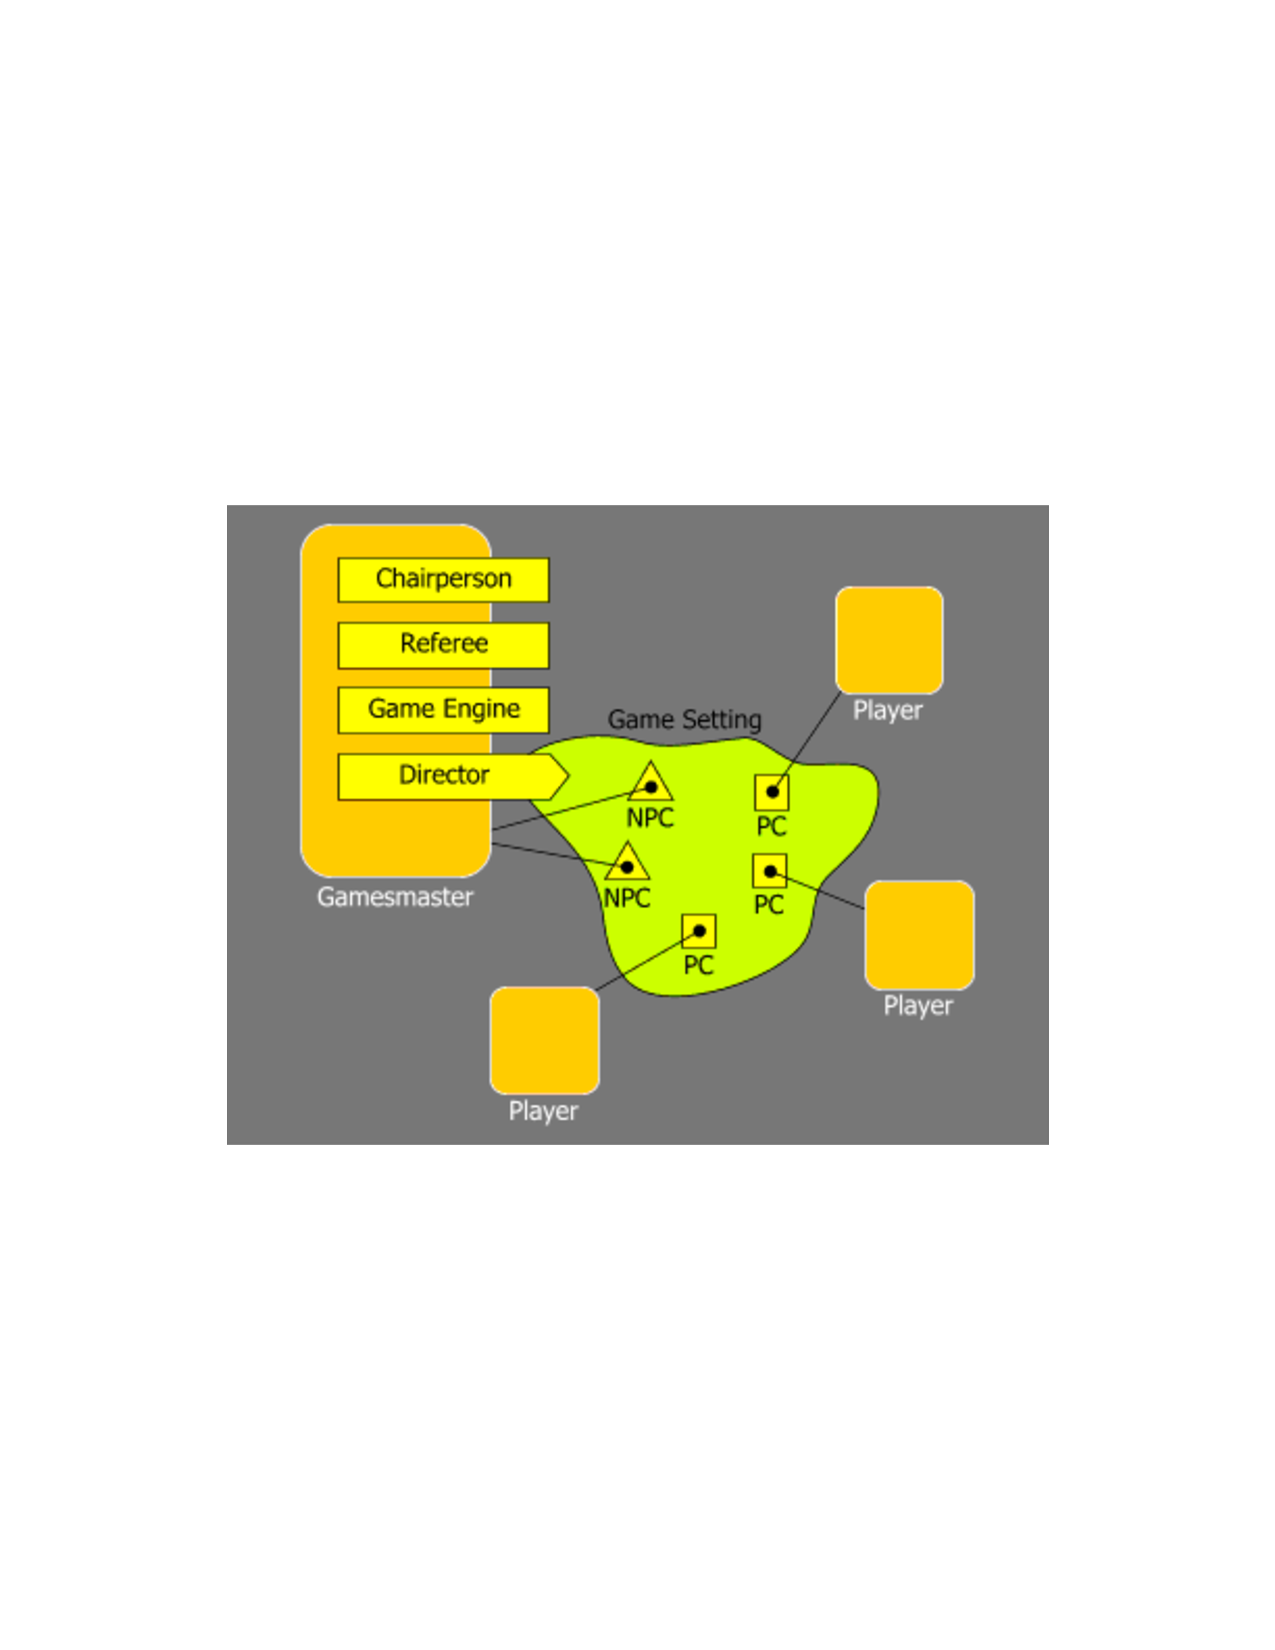
\includegraphics[width=2in]{collaborate_figure1}
\caption{\it A gamesmaster paradigm role-playing game. Each player has a sinlge character, the gamesmaster controlls many non-player characters. In addition the gamesmaster takes the remaining responsibilities in the game.}
\label{gm-paradigm}
\end{figure}
The basic premise of collaborative role-playing is to distribute these responsibilities between all the players. Eventually there comes a point where it doesn't make sense to call one player a gamesmaster any more, this is what gamesmaster-less roleplaying means. All the same jobs are still being done, but they are distributed among all the players.

There are two ways to distribute responsibilities between players. They can be shared or assigned. In principle all of the responsibilities can be shared between two or more players, or assigned to a single player. This means that many different combinations of collaborative-type games can be designed with different ways of distributing each responsibility. The pattern described here is that of the game Ergo; it is a long way from the gamesmaster paradigm, but still attempts to retain playability and iterest.

\section{Step One: Share Responsibility for the Rules}

The first step to collaborative role-playing is to take the game engine responsibility and share it among all players. This comes in two levels.

At the first level everyone shares the task of interpreting the output of the rules. Rather than the gamesmaster interpreting the results of all actions, allow the players to do that when it concerns their character. If one players character rolls to check the success in using a skill, then they should interpret that in game terms. Some information to help them may need to be given by the director, but this is easily accomplished.

The second level is to allow players to generate the inputs to the rules when it affects their character. A character who is using a skill under pressure may need to have a penalty to the player's roll. This penalty can be decided by the player based on their knowledge of the character's personality and experience of the skill and the type of pressure.
\begin{figure}[!htb]
\centering
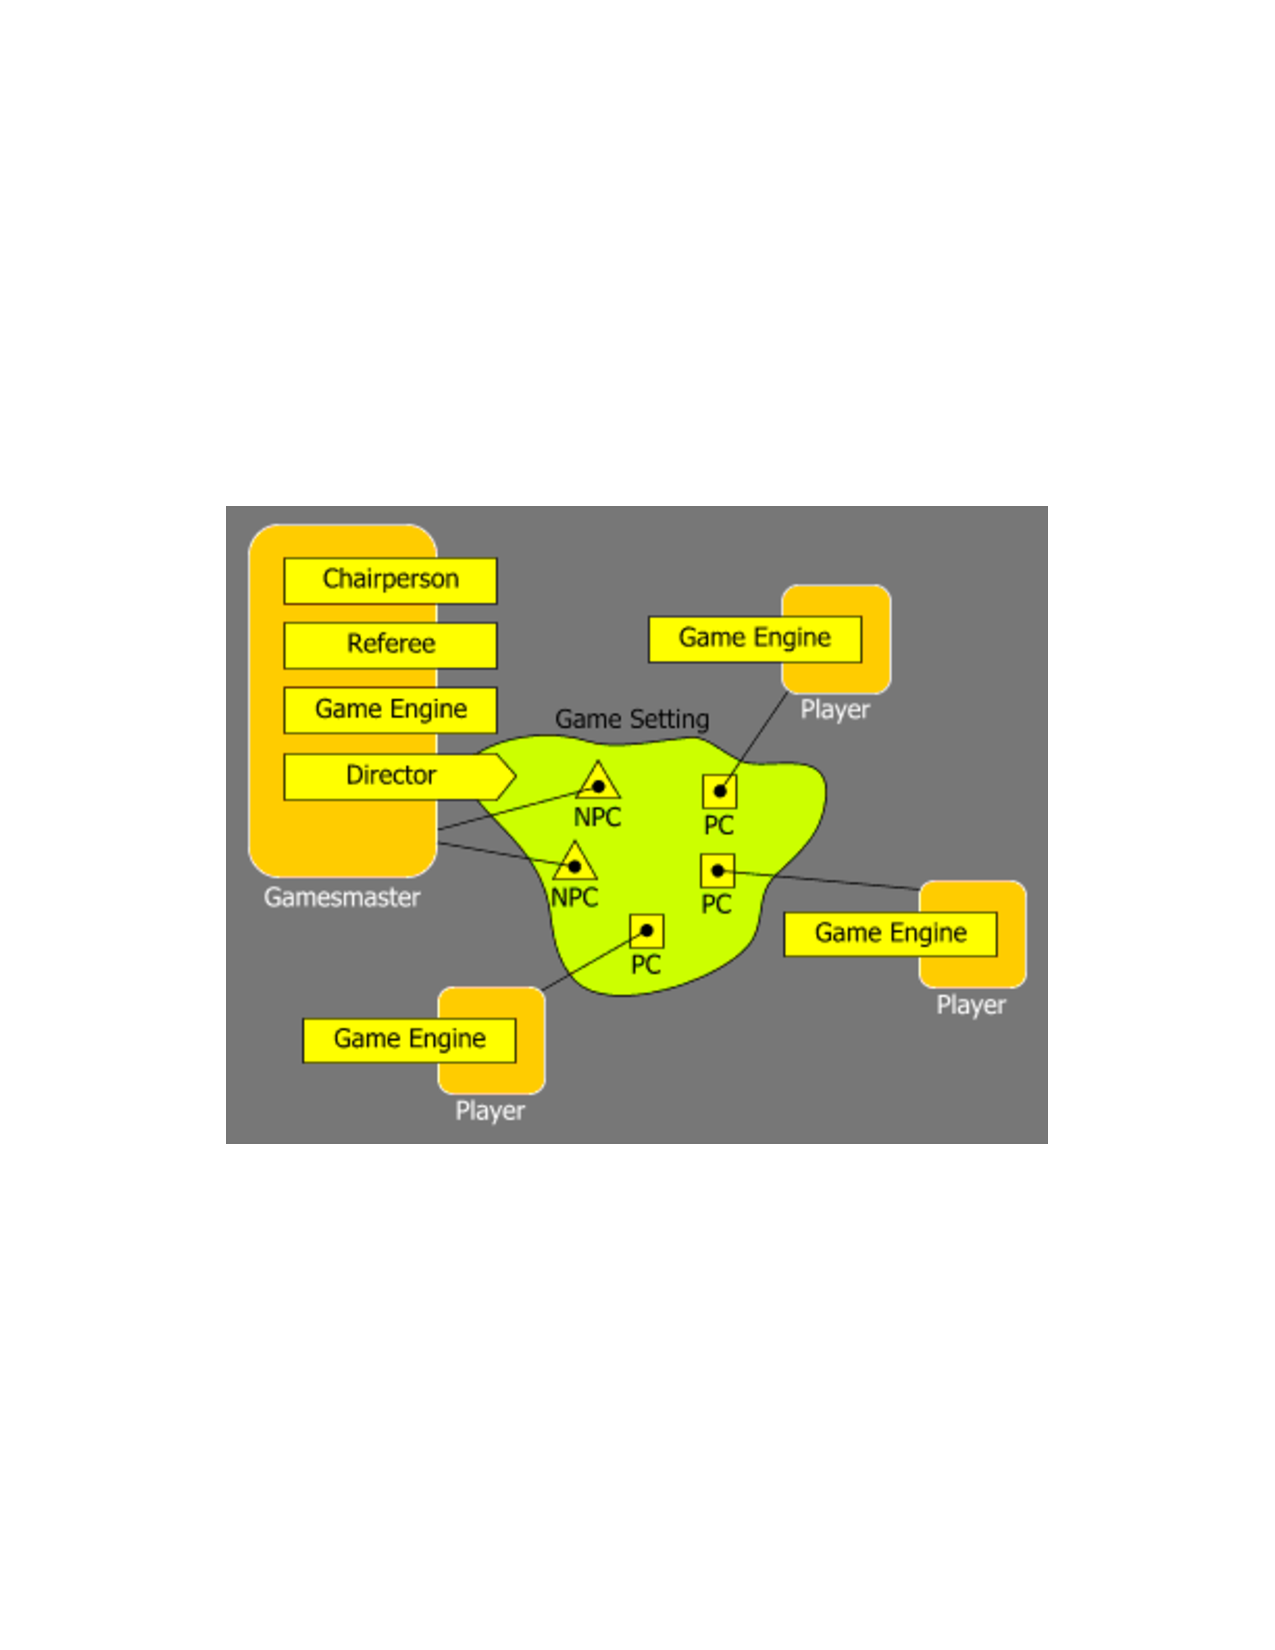
\includegraphics[width=2.5in]{collaborate_figure2}
\caption{\it After step one, every player shares the responsiblity for using the rules. This means being allowed to interpret the results of their characters actions and being allowed to interpret their characters into inputs for the rules.}
\label{players-interpret}
\end{figure}
This is such a simple step from the gamesmaster paradigm that it is quite possible you already do this when playing. Feedback I have received from many different players suggests it is a common adaptation to make. The situation after step one is shown in Figure~\ref{players-interpret}.

\section{Step Two: Share Responsibility for the Story}

This is the most challenging and (in my opinion) the most rewarding stage of moving towards collaborative role-playing. The premise is to share responsibility for the development of the story among all the players. This general scheme is shown in Figure~\ref{fig-distributes}.
\begin{figure}[!htb]
\centering
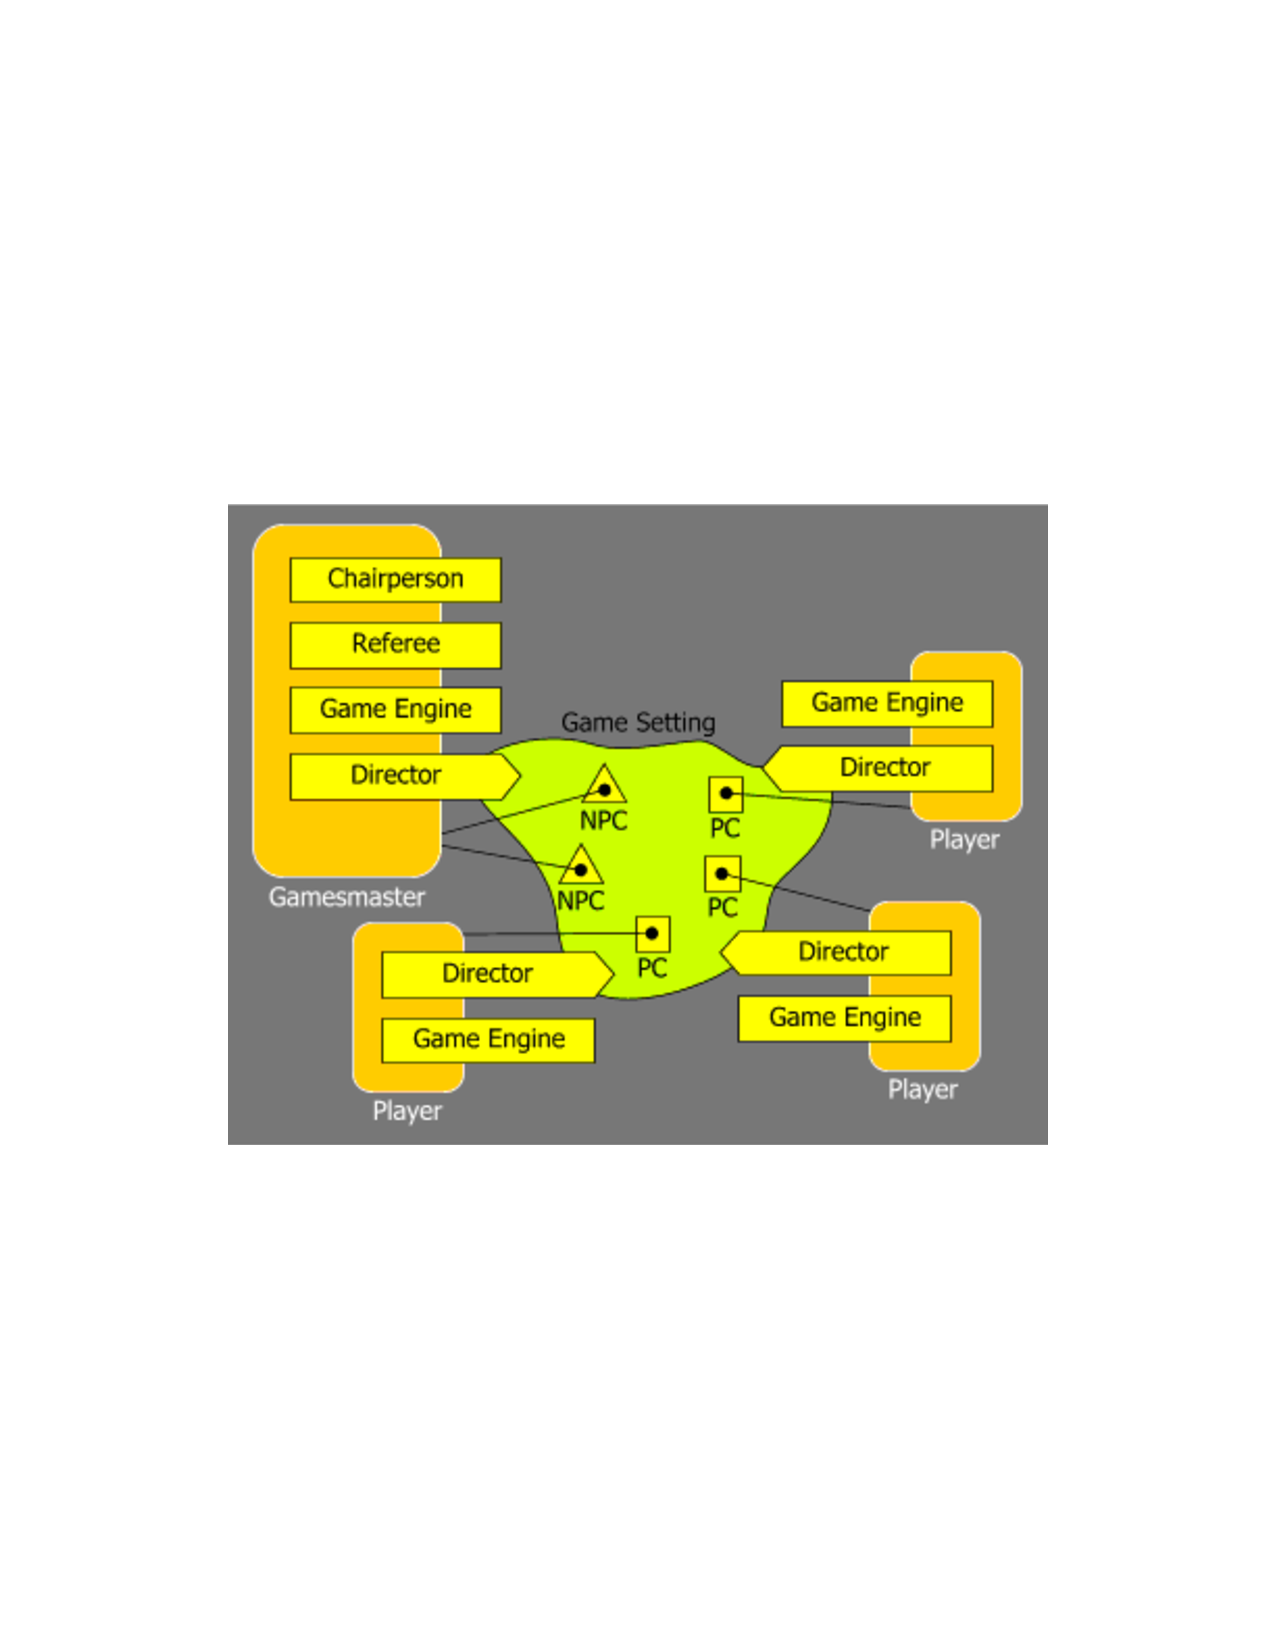
\includegraphics[width=2.5in]{collaborate_figure3}
\caption{\it Step two distributes the responsibility for directing the game among all the players. This may be accomplished in many different ways, depending on the role-players involved.}
\label{fig-distributes}
\end{figure}
Because the directing responsibility is so complex, made up of many different types of job, there are almost unlimited ways to share or assign the responsibility. This stage is where most of the benefits of collaborative role-playing can be found, but also where mistakes can make a game virtually unplayable.

It is beyond the scope of this page to detail all the considerations that should go into distributing this responsibility. The general principle is relatively simple, though.

Directing responsibility that consists of planning a game should be shared among all players. Everyone should participate in planning the game at its most general level, then individual parts of the planning can be assigned to different players when more detail is needed.

In play directing responsibility should be shared between all players but guided by the player or players who planned the relevant sections in the game. So if each player planned a continent, then wherever the characters are based decides who the guide is. In Ergo the guide does not have absolute say, they provide information and guidance so everyone can make decisions. Initially you may choose to make this stronger and give responsibility for the story to the relevant players.

Distributing the story is the hardest and most rewarding part of collaborative play. It does tend to generate more open storylines and can be left out altogether if your group is not suited to such a style of game.

\section{Step Three: Assign Responsibility for the Group}

If you have got this far then the final stage is more symbolic than monumental. The gamesmaster typically has the responsibility for having the ultimate say over what happens in the game and for what happens in the gaming session. Both these responsibilities can be assigned, together or separately, to others. This is shown in Figure~\ref{fig-collab}.

\begin{figure}[htbp]
\centering
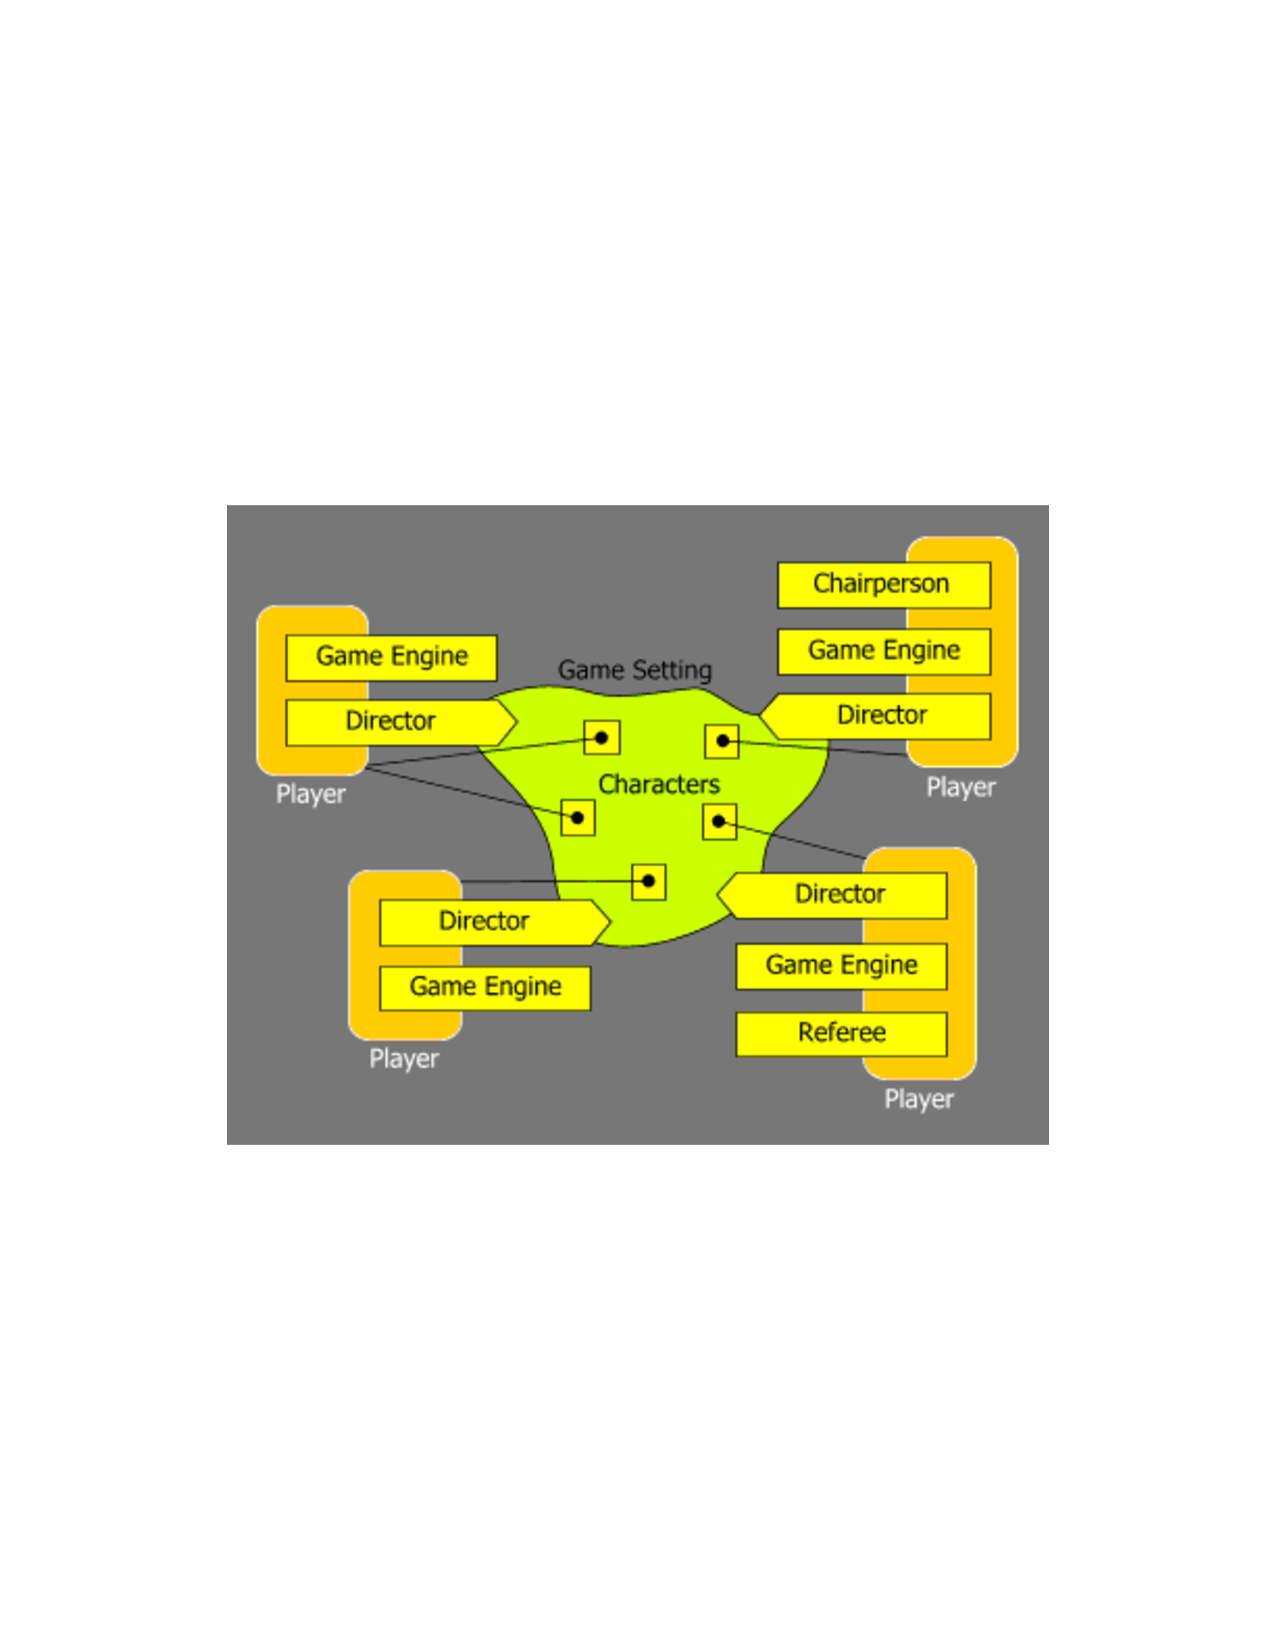
\includegraphics[width=2.5in]{collaborate_figure4}
\caption{\it Finally when the responsibility for chairing the game and refereeing the rules are assigned it makes little sense to call any player a gamesmaster. The game has reached its fully collaborative state.}
\label{fig-collab}
\end{figure}
It is not advisable to try sharing these responsibilities among many players. Such a situation means that social tensions within the group are more likely to arise. Instead assign each responsibility to one player (try to assign the to different players if possible). The responsibilities can be passed between players over many sessions, as long as everyone is clear who has the job at any time.

Some groups are cooperative enough not to need either an explicit chairperson or referee. If this applies to you, then feel free to do without either; the games you play may well be better for it, but take care not to let tensions arise. It is only a game after all.

At this stage it makes very little sense to call any single player a gamesmaster, nor any group of characters player characters or non-player characters. Instead all players have a set of responsibilities, some the same and some different from other players. This is the final destination of collaborative role-playing.


\end{document}

